\documentclass[twocolumn,superscriptaddress,nofootinbib]{revtex4-2}

\usepackage{amsmath} 					
\usepackage{amsfonts}
\usepackage{amssymb} 	
\usepackage{amsthm}
\usepackage{array}       				
\usepackage{graphicx}  					
\usepackage{xcolor}       			
\usepackage{makeidx}   					
\usepackage[utf8]{inputenc} 			
\usepackage{url}     
\usepackage{times}

\usepackage[english]{babel}
	
\usepackage{siunitx}\usepackage{booktabs}
\usepackage{csquotes}
\usepackage[shortlabels]{enumitem}
\usepackage{braket}
\usepackage{tcolorbox}
\usepackage{mathtools}
\usepackage[nolist]{acronym}
\usepackage{tikz}
\usetikzlibrary{quantikz}
\usetikzlibrary{calc}
\pgfdeclarelayer{bg}
\pgfsetlayers{bg,main}

\usepackage{hyperref}

%%%%%%%%%%%%%%%%%%%%%%%%%%%%%%%%%%%%%%%%%%%%%%%%%%%%%%%%%%%
% Environments
%%%%%%%%%%%%%%%%%%%%%%%%%%%%%%%%%%%%%%%%%%%%%%%%%%%%%%%%%%%
\newtheorem{theorem}{Theorem}%[section]
\newtheorem{proposition}{Proposition}%[section]
\newtheorem{definition}{Definition}
\newtheorem{corollary}{Corollary}
\newtheorem{lemma}{Lemma}
\newtheorem{problem}{Problem}
\newtheorem{prescription}{Algorithm}
\newtheorem{algorithm}{Algorithm}
\newtheorem{idea}{Idea}
\newtheorem{observation}{Observation}

\newtheorem{cor}{Corollary}[theorem]
\newtheorem*{remark}{Remark}

\input{commands.tex}

%%%%%%%%%%%%%%%%%%%%%%%%%%%%%%%%%%%%%%%%%%%%%%%%%%%%%%%%%%%
% Other definitions
%%%%%%%%%%%%%%%%%%%%%%%%%%%%%%%%%%%%%%%%%%%%%%%%%%%%%%%%%%%
\DeclareMathOperator{\tr}{tr}
\DeclareMathOperator{\sign}{sign}
\DeclareMathOperator{\poly}{poly}
\DeclareMathOperator{\diag}{diag}
\DeclareMathOperator{\TA}{TA} % Target alignment
\providecommand{\proj}[1]{\ket{#1}\bra{#1}}
\providecommand{\abs}[1]{\lvert #1 \rvert}
\providecommand{\norm}[1]{\lVert #1 \rVert}
\newcommand{\Abs}[1]{\left\lvert #1 \right\rvert}
\newcommand{\Norm}[1]{\left\lVert #1 \right\rVert}
\newcommand{\trace}[1]{\mathrm{tr}\left(#1\right)}
\renewcommand{\l}[0]{\langle}
\renewcommand{\v}[0]{\vert}
\renewcommand{\r}[0]{\rangle}
\newcommand{\dyad}[2]{|#1\rangle \! \langle #2|}

\newcommand{\expval}[1]{\l #1 \r}
\newcommand{\sgn}{\ensuremath{\operatorname{sgn}}}

\newcommand{\X}{\mathcal{X}}
\newcommand{\Y}{\mathcal{Y}}
\newcommand{\R}{\mathbb{R}}



%\newcommand{\id}{\mathbb{I}}
%\newcommand{\ee}{\mathrm{e}}
%\newcommand{\ii}{\mathrm{i}}
%\newcommand{\cc}{\mathbb{C}}
%\newcommand{\EE}{\mathbb{E}}
%\newcommand{\mL}{\mathcal{L}}
%\newcommand{\mV}{\mathcal{V}}
%\newcommand{\mC}{\mathcal{C}}
%\newcommand{\nn}{\boldsymbol{\nu}}
%\newcommand{\bb}{\boldsymbol{b}}
%\newcommand{\order}{\mathcal{O}}

\newcommand{\hc}{\operatorname{h.\!c.}}
\newcommand{\nl}{\lVert}
\newcommand{\nr}{\rVert}

\newcommand{\todo}[1]{\textcolor{red}{[TODO: #1]}}
\newcommand{\jjm}[1]{\textcolor{blue}{#1}}
\newcommand{\pj}[1]{\textcolor{cyan}{#1}}
\newcommand{\tsh}[1]{\textcolor{orange}{#1}}
\newcommand{\egf}[1]{\textcolor{purple}{#1}}
\newcommand{\pf}[1]{\textcolor{green}{#1}}
\newcommand{\dw}[1]{\textcolor{pink}{#1}}

\renewcommand{\AA}{\boldsymbol{A}}
\renewcommand{\aa}{\boldsymbol{a}}

\begin{document}

\title{Trainable Quantum Embedding Kernels for Near-Term Quantum Computers}
\author{Thomas Hubregtsen}
\affiliation{Dahlem Center for Complex Quantum Systems, Freie Universit\"{a}t Berlin, 14195 Berlin, Germany}

\author{David Wierichs}
\affiliation{Institute for Theoretical Physics, University of Cologne, 50937 Cologne, Germany}

\author{Elies Gil-Fuster}
\affiliation{Dahlem Center for Complex Quantum Systems, Freie Universit\"{a}t Berlin, 14195 Berlin, Germany}

\author{Peter-Jan Derks}
\affiliation{Dahlem Center for Complex Quantum Systems, Freie Universit\"{a}t Berlin, 14195 Berlin, Germany}

\author{Paul Fährmann}
\affiliation{Dahlem Center for Complex Quantum Systems, Freie Universit\"{a}t Berlin, 14195 Berlin, Germany}

\author{Johannes Jakob Meyer}
\affiliation{Dahlem Center for Complex Quantum Systems, Freie Universit\"{a}t Berlin, 14195 Berlin, Germany}
\affiliation{QMATH, Department of Mathematical Sciences, University of Copenhagen, 2100 Copenhagen, Denmark}

\date{\today}

\begin{abstract}
Kernel methods are a cornerstone of classical machine learning. The idea of using quantum computers to compute kernels has recently attracted attention for the suitability of these algorithms to be executed on noisy near-term quantum devices. 
Especially kernels arising from embedding data into the Hilbert space of a quantum computer, called \acp{QEK}, have a natural resilience to device noise.
In this work, we address the practical issues arising when realizing Quantum Embedding Kernels on a noisy near-term quantum computer. 
We show under which conditions noise from device imperfections influences the predicted kernel and provide strategies to mitigate these detrimental effects. We also address the influence of finite sampling to provide concentration guarantees.
As an important step towards practical applications, we propose to enrich a Quantum Embedding Kernel with variational parameters. These variational parameters are then adjusted to optimize the alignment of the kernel with respect to the underlying dataset. 
We provide both numerical experiments and tests on actual hardware that showcase the effectiveness of the aforementioned approaches. 
\end{abstract}

\maketitle
\begin{acronym}[UMLX]
    \acro{QEK}{Quantum Embedding Kernel}
    \acro{RBF}{Radial Basis Function}
    \acro{SVM}{Support Vector Machine}
    \acro{ML}{Machine Learning}
    \acro{QML}{Quantum Machine Learning}
    \acro{SDP}{Semi-Definite Program}
    \acro{PQC}{Parametrized Quantum Circuit}
    \acro{NISQ}{Noisy Intermediate-Scale Quantum}
\end{acronym}

\section{Introduction}
In \ac{ML}, Kernel methods are a class of algorithms that employ the kernel trick, which uses the fact that many machine learning algorithms can be written exclusively in terms of dot products between samples \cite{scholkopf2018learning}.  

A challenge arising with kernel methods is that the more expressive models required for complex datasets are in general not efficiently computable.
A proposed solution that to this problem that is of growing interest is the use of quantum computers to calculate kernel matrices, a task they are more suited for than classical computers \cite{heredge2021quantumSVMMeson, bartkiewicz2020ExperimentalKernelFinite, Li2015ExperimentalqSVM}.

A second challenge arising with kernel methods is that of model selection. In classical machine learning, this challenge is overcome by using parametrized kernels, that can be trained via a supervised learning approach \cite{baramLearningPolarization, wangOverviewKernelAlignment2015, cristianiniKernelTargetAlignment2006}. A good kernel model will allow a classifier to identify the correct decision boundaries, as is illustrated in  Fig.~\ref{fig:target_alignment}.

In Quantum Machine Learning, parametrized quantum circuits are used as machine learning models \cite{schuldSupervisedLearningQuantum2018a,wittek2014quantum,lloydQuantumPrincipalComponent2014, schuldEffectDataEncoding2020}. 
In this work, we discuss trainable \acp{QEK}, which employ parametrized quantum circuits to calculate a kernel matrix. 
These \acp{QEK} are then optimized for a specific dataset such that they calculate a kernel matrix for a supervised learning algorithm, such as a \emph{\ac{SVM}}, to enhance its ability to classify the dataset. 
%\cite{schuldQuantumMachineLearning2021} \todo{need some help, need to read paper again}.


\begin{figure}
    \centering
    \includegraphics{figures/front.pdf}
    \caption{Quantum embedding kernels allow for classification of datasets. The quality of classification can be significantly improved by optimizing the parameters of the quantum embedding to increase the target alignment of the kernel.}
    \label{fig:target_alignment}
\end{figure}

\begin{figure*}
    \centering
    \includegraphics{figures/pipeline_two_column.pdf}
    \caption{Schematic of the pipeline used in this work. Green boxes indicate data, purple boxes indicate process steps that are executed on quantum hardware. The pipeline used in this work can be split in three separate parts. In the model selection part, depicted on the left, the parameters of the feature map are adjusted to increase the kernel-target alignment. To calculate the alignment, the kernel matrix is computed and afterwards post-processed to mitigate sampling and device errors. After a sufficient target-alignment is reached, the kernel is used to train a support vector machine. The resulting support vector classifier is used to in the prediction step to label new datapoints.}
    \label{fig:pipeline}
\end{figure*}

In this work, we specifically focus on trainable \acp{QEK} applicable for noisy near-term quantum computers. Since noise must not necessarily be detrimental, for example when using noise mitigation techniques, the proposed methods can be implemented on state-of-the-art hardware. Furthermore, the pipeline introduced in figure \ref{fig:pipeline} can be implemented in a scalable fashion.

    % \todo{contradict advantages? state these as remaining challenges?}
    % \begin{itemize}
    %     \item Con: Noise breaks Mercer Rule for simple overlap estimation protocol.
    %     \item Con: Inherited bad scaling for learning and prediction.
    %     \item Con: Unclear performance, can not test on large datasets yet
    % \end{itemize} 

The rest of this work is organized as follows:
In Section~\ref{sec:kernels} and \ref{sec:quantum_embedding_kernels} we introduce necessary theory relating to classical and quantum embedding kernel methods.
We then describe two types of noise that effect the calculation of kernel matrices in a realistic setting and how they can be dealt with in Section~\ref{sec:the_effects_of_noise}.
In Section~\ref{sec:training_quantum_embedding_kernels}, we introduce how to train \acp{QEK} and present simulation results in Section~\ref{sec:numerical_experiments}, which we obtained using both classical and quantum hardware. 
We conclude by summarizing and discussing our results as well as outstanding question in Section~\ref{sec:summary_and_outlook}.

\subsection*{Notation}
    Before jumping immediately into the body of our work, let us clarify our notation.
    We use bold, lower case letters for vectors such as $\xx$ or $\yy$ and upper case letters for matrices such as $A$ or $B$.
    
    When we look at binary classification tasks, we call our data space $\X\times\Y\subseteq\R^m\times\{-1,+1\}$.
    We refer to $x\in\X$ as $m$-dimensional \emph{points}, and to $y\in\{-1,+1\}$ as corresponding \emph{labels}.
    As usual, we want to approximate some functional relation between $\X$ and $\Y$, but to do so we only have access to a finite size training set
    \begin{align}
        S\coloneqq\{(\xx_1,y_1),\ldots,(\xx_n,y_n)\}\in\left(\X\times\Y\right)^n.
    \end{align}
    Once we have a training set $S$, and when it is clear by context, we will name $\yy\coloneqq(y_1,\ldots,y_n)^\top$ the column vector of labels.
    
    The central tools we use to infer the unknown labeling function are the so-called kernel methods.
    As their name indicates, kernel methods rely heavily on kernel functions, which are commonly denoted with small $k\colon\X\times\X\to\R$.
    Another very important ingredient of kernel methods is the kernel matrix (or Gram matrix), whose job is to list the evaluation of the kernel in every pair of points in our training set $S$.
    We denote it, in turn, as capital $K$:
    \begin{equation}
        K \coloneqq \begin{pmatrix}
            k(\xx_1,\xx_1) & \ldots & k(\xx_1,\xx_n) \\
            \vdots & \ddots & \\
            k(\xx_n,\xx_1) & & k(\xx_n,\xx_n)
        \end{pmatrix},
    \end{equation}
    or, in short, $K_{ij} = k(\xx_i,\xx_j)$ (note kernels are symmetric, so $K_{ij} = K_{ji}$).
    
    In particular, we interest ourselves in families of parameterised kernels.
    One prominent example of such a family is the Gaussian kernel, whose ultimate value depends on a positive parameter $\sigma^2$.
    The families we consider can have arbitrarily many parameters, and we use vector $\ttheta$ to subsume them.
    This way, we write $k_{\ttheta}$ for parameterised kernels and $K_{\ttheta}$ for their respective Gram matrices.

\section{Kernel Methods}\label{sec:kernels}
Kernel methods are among the cornerstones of \ac{ML}.
To understand what a kernel method does, let us first revisit one of the simplest methods to assign binary labels to datapoints: \emph{linear classification}.
    
Imagine we want to discern two different classes of points that lie in different corners of a plane.
A linear classifier corresponds to drawing a line and assigning different labels to the opposing sides of the line, as depicted in Fig.~\ref{fig:linear_classification}.
%
\begin{figure}
    \centering
    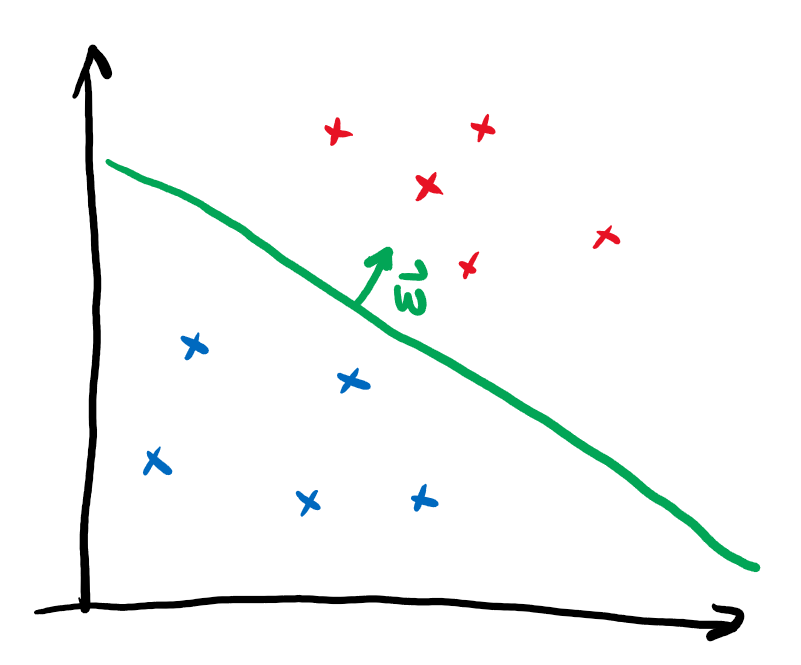
\includegraphics[width=.5\columnwidth]{figures/linear_classification.png}
    \caption{In linear classification, a line (or in higher dimensions a hyperplane) that separates the two classes is sought. We can define the tilt of the line via a vector $\ww$ orthogonal to it.}
    \label{fig:linear_classification}
\end{figure}
%
We can mathematically formalize this notion by assigning the label $y$ to a datapoint $\xx$ via
\begin{align}
   y(\xx) = \sgn(\langle \ww, \xx\rangle + b). 
\end{align}
The vector $\ww$ points perpendicular to the line and thus determines its direction. The intercept term $b$ specifies its position in the plane.
In this form, linear classification can also be extended to higher dimensional vectors $\xx$, where a line is not sufficient to divide the entire space into two regions anymore. Instead, we require a \emph{hyperplane}.
It is immediately clear that this method is not very powerful, as datasets that are not separable by a hyperplane can not be classified with high accuracy using this scheme. 

There is, however, an ingenious way to enhance the capabilities of a linear classifier: if we define some map $\phi(\xx)$ that \emph{embeds} our datapoints into a larger \emph{feature space} and then perform linear classification in this feature space, we could actually realize non-linear classification in the original space of our datapoints. This strategy is visualized in Fig.~\ref{fig:embedding_nonlinear_classification}.
%
\begin{figure}
    \centering
    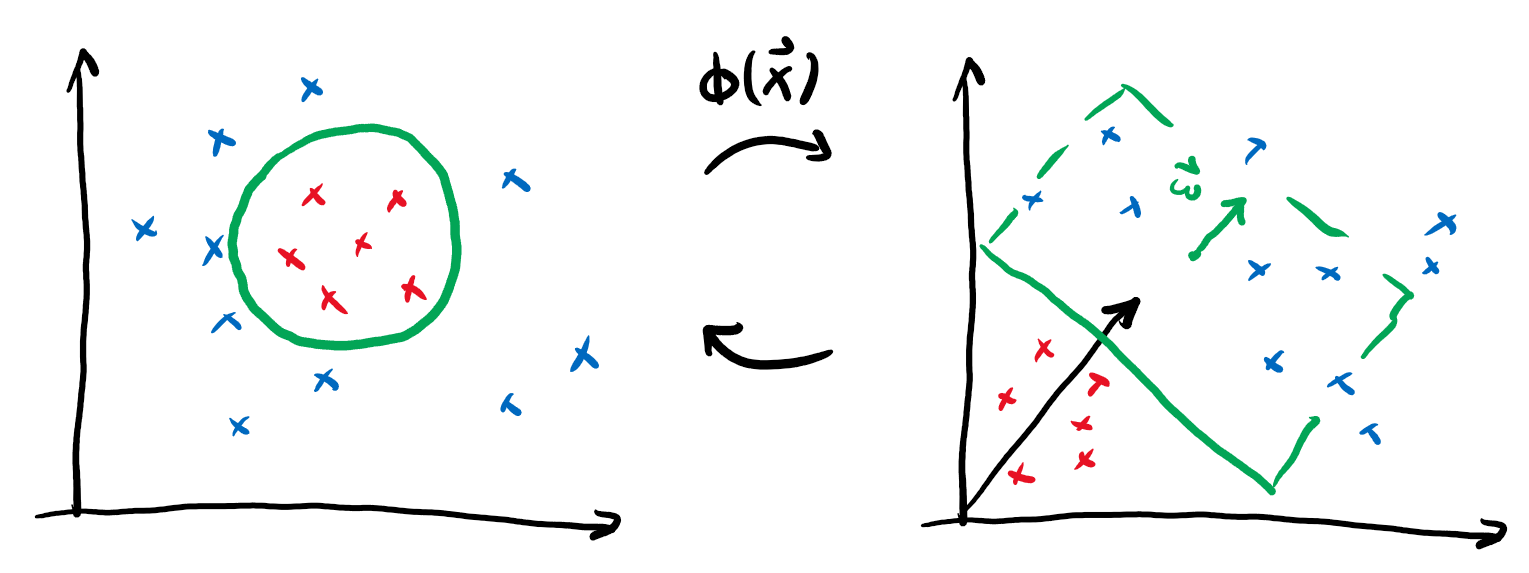
\includegraphics[width=\columnwidth]{figures/embedding_nonlinear_classification.png}
    \caption{A non-linear embedding can be used to enhance the capabilities of a linear classifier. Linear classification in the embedding space can realize non-linear decision boundaries in the original space.}
    \label{fig:embedding_nonlinear_classification}
\end{figure}
%
If include the embedding in the expression for our prediction, we get
\begin{align}\label{eqn:linear_classification_in_feature_space}
y(\xx) = \sgn(\langle \ww', \phi(\xx)\rangle + b),
\end{align}
where $\ww'$ lives in the feature space corresponding to the feature map $\phi$.

A major result in kernel theory is the \emph{representer theorem}~\cite{scholkopf2002learning}. It states that for many ways to quantify the quality of a classifier, we can write the vector $\ww'$ that defines an optimal decision boundary as a sum of the embedded datapoints $\ww' = \sum_i \alpha_i \phi(\xx_i)$. Inserting it into Eq.~\eqref{eqn:linear_classification_in_feature_space} yields
\begin{align}\label{eqn:linear_kernel_prediction}
    y(\xx) = \operatorname{sgn}\left(\sum_i \alpha_i \langle \phi(\xx_i), \phi(\xx)\rangle + b\right).
\end{align}
While this rewriting might not seem useful at first, notice that the above formula only contains inner products between vectors in the embedding space,
\begin{align}
    k(\xx, \xx') = \langle \phi(\xx), \phi(\xx')\rangle.
\end{align}
We call the function $k$ the \emph{kernel} associated to the feature map $\phi$.

The relevant insight is that we can often find an explicit formula for the kernel $k$ making it superfluous to actually perform the embedding $\phi$.
Consider for example the embedding
\begin{align}
    \phi\colon\begin{pmatrix}x_1 \\ x_2 \end{pmatrix} &\mapsto \begin{pmatrix} x_1^2 \\ \sqrt{2} x_1 x_2 \\ x_2^2 \end{pmatrix},
\end{align}
whose associated kernel can be explicitly calculated:
\begin{align}
k(\xx, \yy)
&= \langle \phi\begin{pmatrix}x_1 \\ x_2 \end{pmatrix}, \phi\begin{pmatrix}y_1 \\ y_2 \end{pmatrix}\rangle \\
&= x_1^2 y_1^2 + 2 x_1 x_2 y_1 y_2 + x_2^2 y_2^2 \\
&= (x_1 y_1 + x_2 y_2)^2 \\
&= \langle \xx, \yy \rangle^2.
\end{align}
We find that it can be obtained by simply computing the inner product of two vectors in the initial space and squaring it. Implicitly, we are however computing the inner product relative to the embedding $\phi$! 
This is the central property of kernel-based methods. In many relevant cases the embedding will require a much higher cost to compute than the kernel, while one still gains access the larger feature space through this kernel. This implicit use of the embedding through its associated kernel is known as the \emph{kernel trick}.

If we don't need the embedding at all, how can we then determine if a given function $k$ is actually a kernel for some feature map? This question is answered by checking the \emph{Mercer condition}, which states that any function fulfilling
\begin{align}
    \sum_{i,j} c_i c_j k(\xx_i, \xx_j) \geq 0
\end{align}
for \emph{all} possible sets of real coefficients $\{c_i \}$ and sets of datapoints $\{ \xx_i \}$ is a kernel. Alternatively, we can check whether the kernel matrix $K$ with entries
\begin{align}
    K_{ij} = k(\xx_i, \xx_j)
\end{align}
associated with \emph{any} dataset $\{ \xx_i \}$ is always \emph{positive semidefinite}, i.e.\ that it has no negative eigenvalues.

If we now come back to the example of linear classification in a feature space that motivated our introduction to kernel methods, it is natural to ask how we can best choose the separating hyperplane.
The most popular strategy leads us to the definition of the \ac{SVM}. 
The \ac{SVM} is the application where kernel methods are usually encountered. 
The idea behind \acp{SVM} is to find the hyperplane with the maximal \emph{margin}. 
The margin describes how far you can shift the hyperplane along the vector $\ww$ until you hit a point of the dataset. 
Intuitively, a larger margin is better, since the result would be that outliers of the dataset have a smaller chance of being wrongly classified. 

To predict a class label for a new datapoint, we need to calculate the kernel with respect to the training data points and decide on a class label, as shown in Eq.~\eqref{eqn:linear_kernel_prediction}. A strong advantage of \acp{SVM} is that usually only few weights $\{\alpha_i \}$ contribute significantly to the sum in Eq.~\eqref{eqn:linear_kernel_prediction}. We can thus make a prediction by calculating the kernel with respect to these datapoints from the training dataset. The corresponding datapoints are the eponymous support vectors -- as they support the decision boundary. Intuitively, we can imagine that comparing a new datapoint only to points close to the decision boundary will give important information about the class label.

Kernel methods are not limited to classification. In fact, one can take any machine learning technique that can be reformulated in terms of inner products and replace the inner products by kernel functions to get a \enquote{kernelized} variant. This leads to interesting applications such as kernel principal component analysis~\cite{goos1997kernel} or kernel ridge regression~\cite{saunders1998ridge}.

While we have now seen that kernel methods can enhance the power of many machine learning techniques, the current progress of learning models is not driven by kernel methods but neural networks. This is due to their downsides: For the application of kernel methods, the kernel matrix with respect to the input data needs to be constructed -- which has quadratic complexity in the number of data points. This can already constitute a substantial impediment in the world of big data where the number of datapoints can be in the millions.
Another downside is that the selection of a suitable kernel for a given problem is a non-trivial task. The \emph{\ac{RBF} kernel} also known as \emph{Gaussian kernel} given by
\begin{align}\label{eqn:def_rbf_kernel}
    k_{\text{RBF}}(\xx, \xx') = \exp\left(-\frac{\lVert \xx - \xx' \rVert^2}{2 \sigma^2} \right)
\end{align}
is often a decent starting point, but even there the parameter $\sigma$ that quantifies how close datapoints need to be to be considered similar needs to be fine-tuned. 
%In this work we will address this drawback by using a measure of agreement between the dataset and the kernel, the so-called \emph{kernel-target alignment}, to train variational parameters of the kernel to increase its fitness on a dataset. % jjm: doesn't really fit here

Despite the fact that kernel methods do not dominate contemporary machine learning applications, they are extremely useful to understand learning models in general. This is because many learning methods can be mapped back to kernel methods for which in turn there exist theoretical guarantees, for example on their capability to generalize on unseen data~\cite{scholkopf2002learning}.
    
\section{Quantum Embedding Kernels}\label{sec:quantum_embedding_kernels}

On \ac{NISQ} hardware, we need to make use of quantum gates, like Pauli rotations, to load data onto the quantum computer. This constitutes a full quantum circuit that is represented by a unitary dependent on the specific datapoint, $U(\xx)$. As soon as the data is loaded, the quantum system is in a state that depends on the datapoint in question, 
\begin{align}
    \ket{\phi(\xx)} = U(\xx) \ket{0}.
\end{align}
This approach is also known as a \emph{quantum feature map}~\cite{schuld2019quantum_feature_hilbert_space} because we are effectively embedding the datapoint in the Hilbert space of quantum states.
As we learned in Sec.~\ref{sec:kernels}, it is no large step from a feature map to a kernel function. We only need to take the inner product between quantum states, which is given by the \emph{overlap}
\begin{align}\label{eqn:qek_pure_state}
    k(\xx,\xx') &= \abs{\braket{\phi(\xx')|\phi(\xx)}}^2.
\end{align}
This is the \emph{\acf{QEK}} associated to the quantum feature map $\ket{\phi(\xx)}$. 

In general, we will not be able to avoid noise, which means that we can not assume that the embedded quantum state is pure. In this case, the quantum embedding is realized by a data-dependent density matrix $\rho(\xx)$, which for a pure state reduces to $\rho(\xx) = \dyad{\phi(\xx)}{\phi(\xx)}$. The inner product, which is still corresponds to the overlap, is given by
\begin{align}\label{eqn:qek_mixed_state}
    k(\xx,\xx') = \Tr\{\rho(\xx)\rho(\xx')\}.
\end{align}
This inner product is also known as the Hilbert-Schmidt inner product for matrices. For pure quantum states, this reduces to Eq.~\eqref{eqn:qek_pure_state}.

In summary, every quantum feature map induces a quantum embedding kernel. We can use this kernel as a subroutine in a classical kernel method, for example the \ac{SVM}, which makes for a hybrid quantum-quantum classical approach. In this case, the separating hyperplane is constructed in a purely classical manner, only the kernels between the training datapoints are evaluated on the quantum computer. 

To be able to use quantum embedding kernels in this way, we need to evaluate the overlap of two quantum states on near-term hardware. There are a number of algorithms to estimate the overlap of two quantum states ~\cite{fanizzaSwapTestOptimal2020,buhrman2001QuantumFingerprinting,Cincio2018LearningAlgorithmStateOverlap,huang2020predicting}, all of which are agnostic to how the states were obtained. This means we can do better by exploiting the specifics of this setting.

For pure embedding in particular, this is straightforward if we can construct the adjoint of the data-encoding circuit, $U^\dagger(\xx)$. In this case, we can rewrite the overlap as
\begin{align}\label{eq:ancilla_free}
    \abs{\braket{\phi(\xx')|\phi(\xx)}}^2 = \abs{\braket{0|U^\dagger(\xx')U(\xx)|0}}^2.
\end{align}
This is nothing else but the probability of observing the $\ket{0}$ state when measuring the state $U^\dagger(\xx')U(\xx)|0\rangle$ in the computational basis.
In order to obtain an estimate, we can therefore initialize the quantum system in the $|0\rangle$ state, apply the unitary operation $U(\xx)$ followed by $U^\dagger(\xx')$, and finally measure in the computational basis.
From there, we only need to record the frequency with which the prepared state is found in the $\ket{0}$ state to obtain our estimate.
The circuit diagram for this \emph{ancilla-free} approach can be found in Fig.~\ref{fig:ancilla_free}. The advantage of this scheme is that it does not need additional qubits, but it doubles the circuit depth.

\begin{figure}
    \centering
    \begin{quantikz}
    \lstick{$\ket{0}$}&\gate{\vphantom{\int}U(\xx)}&\gate{\vphantom{\int}U^{\dagger}(\xx')}& \meterD{\vphantom{\int}\lvert 0\rangle\!\langle 0\rvert}
    \end{quantikz}  
    \caption{The overlap between the embedded states can be computed by applying the unitary $U(\xx)$ embedding the first datapoint and the adjoint of the unitary embedding the second datapoint $U^{\dagger}(\xx')$. This approach results in a doubled circuit depth but does not need ancillas. It works only for pure states.}
    \label{fig:ancilla_free}
\end{figure}

Another alternative approach to estimate the overlap between two quantum states is the \emph{SWAP test}. The SWAP test is based on the \emph{SWAP trick}, a mathematical gimmick that allows us to transform the product of the density matrices in Eq.~\eqref{eqn:qek_mixed_state} into a tensor product:
\begin{align}
    k(\xx, \xx') &= \Tr\{\rho(\xx)\rho(\xx')\} \\
    &= \Tr \{ (\rho(\xx) \otimes \rho(\xx')) S \},
\end{align}
where $S$ denotes the SWAP operation between the two quantum systems in the states $\rho(\xx)$ and $\rho(\xx')$. To extract this quantity, the SWAP test makes use of an ancillary qubit that controls the SWAP operation. The exact circuit is depicted in Fig.~\ref{fig:swap_test}. While this approach is not ancilla-free and needs a larger quantum computer it does only slightly increase the depth of the overall circuit and it also works for mixed quantum states.

\begin{figure}
    \centering
    \begin{quantikz}
    \lstick{$\ket{0}$}&\gate{H}&\ctrl{2}&\gate{H}&\meterD{Z}  \\
    \lstick{$\ket{0}$}&\gate{U(\xx)}&\swap{1}&\qw&\qw  \\
    \lstick{$\ket{0}$}&\gate{U(\xx')}&\targX{} &\qw&\qw
    \end{quantikz}  
    \caption{The overlap between the embedded states can be computed by embedding both datapoints in parallel. An ancillary qubit is then used together with controlled SWAP operations to extract the overlap, which is obtained from the expectation value of the Pauli-$Z$ observable on the ancilla. This approach results in a doubled circuit width and requires one ancilla and controlled SWAP operations. It works for pure and mixed states.}
    \label{fig:swap_test}
\end{figure}

As quantum feature maps are indispensable in NISQ computing, it is no surprise that quantum embedding kernels are instrumental beyond their use as subroutines for classical machine learning methods. In Ref.~\cite{schuldQuantumMachineLearning2021} it was shown that all variational quantum learning methods boil down to kernel methods, providing an opening for kernel theory to explore the properties of these learning models.


\section{Training Quantum Embedding Kernels}\label{sec:training_quantum_embedding_kernels}
Quantum feature maps can have variational parameters. In this section, we discuss how to adjust these parameters to improve the classification capabilities of quantum embedding kernels.

Before we can dive into the details we take a step back to clear up the terminology we use in this work. Adjusting the variational parameters of a quantum feature map -- and therefore of its associated quantum embedding kernel -- can be seen as a particular instance of \emph{model selection}. For our purposes, we again split this into two steps, first \emph{kernel selection} and second \emph{kernel optimization}. Kernel selection means choosing a particular quantum circuit layout with variational parameters that are not yet 

\subsection{Kernel selection and kernel optimization}\label{ssec:model_selection}
    
    In kernel-based \ac{ML}, finding the optimal values for a parametrized kernel is seen as a model selection task.
    For our case of interest, model selection is a two-step process: \emph{kernel selection} and \emph{kernel optimization}.
    Kernel selection is fixing a (parametrized) kernel function family, as for instance the Gaussian kernel in classical \ac{ML}.
    Then, kernel optimization is the process of fixing a value for the parameters, which could be as simple as a greedy search in parameter space.
    Kernel-based model selection is not far from Neural Network-based model selection in spirit.
    With Neural Networks, first we fix the architecture and hyperparameters (kernel selection) and then we learn the best parameters (kernel optimization).

    Selecting the right kernel and finding good parameters is of course key.
    The kernel function fixes the geometry of the Hilbert Space onto which data is embedded.
    The geometry inherited from different kernels can then become either a catalyst or a caveat to linear separability on feature space\footnote{
    For instance, one can take the Gaussian kernel and check the asymptotic behavior $\sigma^2\to\{0,\infty\}$ as Ref.~\cite{keerthiLin} did.
    Even without performing their rigorous study it should be clear very small or very large parameter values yield poor results.}, which is our final goal.
    
    We now turn ourselves to the object of our study: \acp{QEK}.
    We can interpret Sec.~\ref{sec:quantum_embedding_kernels} as setting the grounds for kernel selection.
    In particular, we propose studying kernels arising from parametrized circuits.
    Kernel selection here refers to designing the circuit architecture, namely which specific gates we use and where in the circuit they show up.
    Since one usually picks general Pauli rotations, we can understand the parameters as rotation angles.
    Following the jargon, kernel optimization would be fixing these angles with the goal of enabling linear separation on feature space.
    
    Next we propose a cost function with which we can train the parameters.
    
\subsection{Kernel Target Alignment}\label{ssec:target_kernel_alignment}

    Our goal is to learn which parameter values to use based on given data.
    We therefore need some measure to assess the quality of different kernels.
    Early approaches involved some variant of exhaustive parameter search, where at each iteration the quadratic optimization program tied to fitting an \ac{SVM} had to be solved \todo{cite? This is pretty standard}.
    An example of such an approach is the ``leave-one-out" error bound \cite{scholkopf2002learning}, where after training the \ac{SVM} with all points but one, the predicted label for the left out point describes the quality of the kernel.
    However, this measure, as well as other common contemporary approaches carry a large runtime complexity, and are thus only suitable for tuning few parameters.
    
    One would hope for efficiently computable and universal kernel evaluation measures, which could act as a predictor of classification accuracy without involving costly computations.
    Luckily enough, Ref.~\cite{wangOverviewKernelAlignment2015} walks us through a number of such measures as proposed in  Refs.~\cite{cortes2012CenteredAlignment, baramLearningPolarization, wang2009LocalKernelPolarization, Wang2008KernelClassSeparability, xiong2005EmpiricalFeatureSpace, nguyen2008kernelmatrixevaluationmeasure}, using the \emph{Kernel Target Alignment} from Ref.~\cite{cristianiniKernelTargetAlignment2006} measure as central element.
    Two shared properties of all these measures are: (1) they can be computed efficiently, and (2) the information from the entire training set $S$ is used in evaluating them.
    One reason for sticking to the Target Alignment is that it has a clear geometric interpretation, which we see below.
    Also, despite its simplicity, Target Alignment benefits from theoretical guarantees regarding both its high concentration about the expected value and its good generalization behavior in labeling previously unseen data \cite{cristianiniKernelTargetAlignment2006, kandola2002optimizingalignmentcombinations,nguyen2008kernelmatrixevaluationmeasure}.
    
    Let us now define this quantity.
    It is at this point helpful to notice that we can understand matrices as vectors.
    One way of ``vectorizing" a matrix $B$ is to write the rows one after the other, resulting in a $1$-dimensional object we can name $\bb$:
    \begin{align}
        \bb = (B_{11},\ldots,B_{1n},B_{21},\ldots,B_{2n},\ldots,B_{nn}).
    \end{align}
    In this picture, we can take the usual inner product of vectors:
    \begin{align}
        \langle\bb,\bb'\rangle = \sum_k b_k b'_k = \sum_{i,j} B_{ij}B'_{ij}.
    \end{align}
    This inner product is called the Frobenius inner product, and it is a common inner product to take when working with vector spaces of matrices.
    Formally, the Frobenius inner product of two $n\times n$ matrices $B$ and $B'$ is defined as
    \begin{equation}
        \langle {B,B'} \rangle_F \coloneqq \sum_{i,j=1}^n B_{ij} B'_{ij},
    \end{equation}
    
    One can now also define the Frobenius norm of matrix $B$ as
    \begin{align}
        \Norm{B}_F \coloneqq \sqrt{\langle B,B\rangle_F}.
    \end{align}
    
    Recall the inner product of two vectors is a natural measure of how similar the direction of both vectors is.
    One usually learns $\langle\vv,\ww\rangle=\Norm{\vv}\Norm{\ww}\cos{\vartheta}$, where $\vartheta$ is the angle described between both vectors.
    In much the same way, we can use the Frobenius inner product and Frobenius norm of two matrices $B$ and $B'$ to assess how similarly aligned they are.
    Concretely, the alignment between two matrices $B$, $B'$ is
    \begin{equation}
        \operatorname{A}(B, B') \coloneqq \frac{\langle B, B'\rangle_F}{\Norm{B}_F \Norm{B'}_F}.
    \end{equation}
    One notices $\operatorname{A}$ plays the role of the cosine between the matrices.
    Consequently, the alignment and the Frobenius distance of two matrices are closely related:
    \begin{align*}
        \Norm{B-B'}_F^2 =\Norm{B}_F^2 +\Norm{B'}_F^2 - 2\operatorname{A}(B,B') \Norm{B}_F \Norm{B'}_F
    \end{align*}
    
    The evaluation measure we use is starkly rooted in the cosine between matrices.
    Computing the alignment of two kernel matrices tells us how similar both kernels are on feature space.
    Our strategy consists on defining an \emph{ideal target matrix} from the training data, and then find a kernel with high similarity to it.
    We can define the ideal target matrix $K^\ast$ as the outer product of the data label vector $\yy$ with itself $K^\ast = \yy\yy^\top$.
    Since $K^\ast$ is an outer product, it is positive semi-definite.
    It follows that the ideal target matrix can also be viewed as a kernel, whose kernel matrix is $K^\ast_{ij}=y_i y_j$.
    The \emph{Kernel-Target Alignment} of a kernel is defined as the alignment between the Gram matrix on the points and the ideal target matrix from the labels
    
    \begin{align}
        \TA(k) = \operatorname{A}(K,K^\ast).
    \end{align}
    
    When computing $\TA$ we can make use of the fact that $K^\ast = \yy\yy^\top$, leading to
    \begin{align}
        \TA(k) & = \frac{\langle K,\yy\yy^\top\rangle_F}{\Norm{K}_F\Norm{\yy\yy^\top}_F} \\
        & = \frac{\sum_{i,j=1}^n k(x_i,x_j)\,\, y_i y_j}{n \Norm{K_F}} \label{eq:polarisation}\\
        & = \frac{\yy^\top K\yy}{n \Norm{K}_F},
    \end{align}
    where we used $\Norm{\yy\yy^\top}_F = n$. \todo{Introduce the rescaling of $y_i$ for unbalanced datasets here}.
    
    If we pay close attention to the numerator in Eq.~\ref{eq:polarisation}, we can gather further intuition for why $\TA$ is a meaningful measure.
    Each term $y_iy_j \, k(\xx_i,\xx_j)$ in the sum is a product of the kernel function of two points and their labels.
    If both points belong to the same class $y_i=y_j$, the kernel value will add to $\TA$, whereas if the labels are different $y_i=-y_j$, the term will contribute negatively to the overall sum.
    Maximizing the sum then means both, maximizing the kernel values for pairs of points in the same class ($y_i=y_j$) and minimizing the kernel values between points with opposite labels ($y_i=-y_j$).
    
    Geometrically, the kernel is maximal if the points in feature space are identical and is minimal, i.e.~vanishes, if they are orthogonal to one another.
    Let us assume we are able to reach perfect alignment.
    In feature space this would mean all elements of a class concentrate in a single point, because all elements with the same label must fulfill $k(\xx_{\{y\}},\xx'_{\{y\}}) = 1$.
    Also, the kernel must vanish for any pair of points belonging to different classes $k(\xx_{\{y\}},\xx_{\{-y\}}) = 0$.
    This orthonormality between points of distinct classes ensures linear separability.
    Taking one step back and looking at the entire picture again, we understand how maximizing the Kernel Target Alignment could ensure good linear separability.
    
    One question remains, and that is how we can maximize the Target Alignment.
    But remember this is independent of training the \ac{SVM}, we are still in the process of model optimization!
    By this point, some parametrized embedding ansatz for the \ac{QEK} is assumed to be already selected.
    We must find the optimal values for the rotation angles, and we can do it via a number of ways.
    The setting is inviting for gradient-based optimization, where we iterate over $\ttheta$ values according to some update rule.
    By repeating this step we are eventually left with the approximately optimal parameters $\ttheta^\ast$.
    We close the kernel optimization phase when we fix the kernel to be $k=k_{\ttheta^\ast}$.
    After this last step we can forget the kernel was trainable altogether and go on to pick a classifier as is done in classical \ac{ML}.
    
    There is one important final remark regarding the Target Alignment trainability.
    As opposed to some of the earlier kernel quality estimators, the Target Alignment is differentiable with respect to the kernel parameter vector $\ttheta$.
    We do not spell out the analytical gradient nor the update rule, but Refs.~\cite{camargo2009MulticlassKernelAlignment,guermeur2004KernelProtein,igel2007GradientOptimizationKTAlignment,Pothin2006GreedyOptimizingKernelAlignment,Pothin2007FeatureRepresentationKTAlignment} showed how the task of finding
    \begin{equation}
        \ttheta^\ast = \operatorname{arg}\max_{\ttheta} \TA(k_{\ttheta})
    \end{equation}
    is well posed in terms of convergence via gradients.
    
    \jjm{
        Optimizing kernels using the kernel-target alignment as a cost function is closely related to the approach put forward for the training of quantum feature embeddings of Ref.~\cite{lloyd2020QuantumEmbeddingsML}. The authors suggest to train an embedding $\ket{\phi_{\ttheta}(\xx)}$ by optimizing the Hilbert-Schmidt distances between the embedded data points in the two classes. These are modeled via the mixed states obtained from averaging over all embedded datapoints:
        \begin{align}
            \rho_{\pm}(\ttheta) &= \frac{1}{|\calS_{\pm}|} \sum_{\xx \in \calS_{\pm}} | \phi_{\ttheta}(\xx) \rangle \! \langle \phi_{\ttheta}(\xx) | \\
            &= \frac{1}{|\calS_{\pm}|} \sum_{\xx \in \calS_{\pm}} \phi_{\ttheta}(\xx) ,
        \end{align}
        where we denoted subsets of the dataset corresponding to the labels $+1$ and $-1$ as $\calS_{+}$ and $\calS_{-}$, respectively and introduced the shorthand $\phi_{\ttheta}(\xx)$ for the density matrix associated to the embedded state. The objective function is then given by
        \begin{align}
            P(\ttheta) = \Tr\{(\rho_{+}(\ttheta) - \rho_{-}(\ttheta))^2 \}.
        \end{align}
        The relation to kernel-target alignment becomes apparent if we consider that we can rewrite the numerator of the kernel-target alignment -- the polarization -- in terms of these density matrices. To see this we consider the polarization:
        \begin{align}
            \sum_{i,j=1}^N y_i y_j k_{\ttheta}(\xx_i, \xx_j)
            &= \sum_{i,j=1}^N y_i y_j \langle \phi_{\ttheta}(\xx_i), \phi_{\ttheta}(\xx_j) \rangle \\
            &= \left\langle \sum_{i=1} y_i \phi_{\ttheta}(\xx_i), \sum_{i=1} y_i \phi_{\ttheta}(\xx_i) \right\rangle.
        \end{align}
        We see that the polarization is nothing else but the square of the induced norm of the sum of the embeddings weighted by the labels. For a \ac{QEK}, this is nothing else but the difference of the two density matrices introduced above:
        \begin{align}
            \sum_{i=1} y_i \phi_{\ttheta}(\xx_i) &= \rho_{+}(\ttheta) - \rho_{-}(\ttheta).
        \end{align}
        As already noted by the authors of Ref.~\cite{lloyd2020QuantumEmbeddingsML}, the polarization can be rewritten as
        \begin{align}
            P(\ttheta) = \Tr\{\rho_{+}(\ttheta)^2 + \rho_{-}(\ttheta)^2 - 2 \rho \sigma \}.
        \end{align}
        This means that increasing the polarization means increasing the purity of the data embedding states [need better name]  $\Tr \{ \rho_{\pm}(\ttheta)\}^2$, thereby encouraging the points in the dataset to cluster closer together and at the same time decreasing the overlap of the two data embedding states, thereby encouraging them to reside in different corners of the Hilbert space.
        We think, however, that the kernel-target alignment -- representing the normalized polarization -- is a measure that is easier to interpret and more accessible to numerical optimization than the pure polarization. 
        The authors of Ref.~\cite{lloyd2020QuantumEmbeddingsML} use the trained embeddings to perform a classification based on the fidelity with the data embedding states $\rho_{\pm}$, which corresponds to a kernelized nearest-centroid classification. The use of the embedding as a \ac{QEK} in a support vector machine therefore allows for more sophisticated decision boundaries.
    }
    
\section{The Effects of Noise}
\label{sec:the_effects_of_noise}
\subsection{Device Noise}

Near-term quantum devices suffer from unavoidable noise caused by unintentional interactions with the environment or imperfect control. 
It is therefore impossible to prepare pure quantum states with an embedding circuit. 
This fact has multiple implications for our kernel methods and their implementation.

When performing the SWAP test, the noise -- while reducing the quality of the produced states and their overlap -- does not lead to any conceptual problems with the \ac{QEK}, in particular the kernel remains positive semi-definite.
In our approach, however, the adjoint of the embedding is required (see Eq.~\eqref{eq:ancilla_free}).
While the operations in the (perfect) embedding circuit are unitary and typically the inverse -- and thus the adjoint -- of all elementary operations are available, the circuit noise can in principle prevent us from implementing the adjoint embedding.
As an example consider a noisy channel $\calV(\theta)$ modeled by a rotation gate $R(\theta)$ that is followed by a noise channel $\calN$:
\begin{align}
    \calV[\rho] = \calN[R(\theta) \rho R^{\dagger}(\theta)].
\end{align}
For a standard rotation gate, we have $R^\dagger(\theta)=R(-\theta)$ and can write
\begin{align}
    \calV[\rho] = R(-\theta) \calN^\dagger[\rho ] R^{\dagger}(-\theta).
\end{align}
We see that the adjoint of the channel requires us to implement the adjoint noise channel $\calN^\dagger$ and that the order of the noise channel and the unitary is changed.
As the noise model resembles unintentional effects in the quantum device, we should not expect sufficient control to implement the adjoint or realize a channel that corrects for the changed order of operations. Instead, we require assumptions on the noise channel, namely that it is self-adjoint ($\calN=\calN^\dagger$) and that it commutes with the unitary circuit operation.
Under these assumptions, the ancilla-free approach is equivalent to the SWAP test and yields a positive semi-definite kernel matrix. 

It turns out that near-term quantum devices can be described sufficiently well by noise models that satisfy the assumptions above, e.g.~depolarizing noise and random control noise in rotation gates.
While these models yield a realistic description, tracing and correcting for each single error they introduce to the circuit is typically intractable.
Therefore we will present a mitigation technique for the kernel matrix based on a simpler noise model and investigate its performance on both, a realistic noisy simulation and quantum hardware.

% For the \emph{ancilla-free} approach, however, we have to make some assumptions on the properties of the noise. Let us first consider the general setting for a noisy circuit. We want to estimate the overlap between two noisy quantum states, which allows us to reformulate

% From these manipulations it is apparent that we have to implement the \emph{adjoint} of the embedding channel $\Phi$ in order to compute the overlap between the two noisy states. This poses a problem: while we can implement the adjoint of perfect unitaries, we usually do not have access to the adjoints of imperfect unitaries. Often, noisy gates on near-term devices can be modeled by a perfect unitary followed by some kind of noise channel $\calN$,
% \begin{align}
%     \calV(\phi)[\rho] = \calN[U(\phi) \rho U^{\dagger}(\phi)] = (\calN \calU(\phi))[\rho] .
% \end{align}
% In this case, the adjoint is given by
% \begin{align}
%      (\calN \calU(\phi))^{\dagger} = \calU^{\dagger}(\phi) \calN^{\dagger}.
% \end{align}
% We see that both the order changes and that we now have the adjoint of the noise channel contributing. We must now implement this operation with the noisy gates available on the device. Here, the inversion of $\calU(\phi)$ is usually straightforward, as for example for rotation gates we have that $\calU^{\dagger}(\phi) = \calU(-\phi)$. But this is not enough for a faithful reproduction as we also need to maintain order. We note that
% \begin{align}
%     \calV(-\phi) &= \calN \calU^{\dagger}(\phi) \\
%     &\neq \calU^{\dagger}(\phi) \calN^{\dagger} \\
%     &= \calV^{\dagger}(\phi).
% \end{align}
% This means that the figure of merit that determines how well we can evaluate an overlap by \emph{umcomputing} is essentially how closely we can approximate $\calV^{\dagger}(\phi)$ with noisy gates available on our device. As variational circuits are usually composed from rotation gates and $\calU(-\phi)$ is the adjoint of $\calU(\phi)$, $\calV(-\phi)$ is the obvious and cheapest way of realizing $\calV^{\dagger}(\phi)$ approximately.
% A quality measure for the approximation is the diamond norm distance
% \begin{align}
%     \lVert \calV^{\dagger}(\phi) - \calV(-\phi) \rVert_{\diamond}.
% \end{align}

% Luckily, there is a regime in which $\calV^{\dagger}(\phi) = \calV(-\phi)$ holds, namely when the noise is self-adjoint, i.e., $\calN = \calN^{\dagger}$ (as is the case for all Pauli noise channels and random unitary channels), and commutes with $\calU(\phi)$. This is not an unrealistic assumption, as many near-term quantum computers can be described suitably well by a depolarizing noise model which has these properties. Another such noise model is control noise originating from random over- or underrotations which is self-adjoint and by definition commutes with the underlying rotation implemented.

\subsubsection{Mitigating Depolarizing Noise} \label{sec:device_noise_mitigation}
As mentioned above, depolarizing noise is often a suitable noise model for near-term devices and at the same time allows us to implement the adjoint embedding and therefore to use the ancilla-free approach.
However, as this noise channel is not unitary, we do not invert the noise when using the adjoint embedding but inflict additional noise instead.

We know that a perfect circuit would yield the outcome $1$ for all diagonal entries of the kernel matrix $K$. While we can use this knowledge to save quantum computational cost, it might be more valuable to compare the output of the quantum computer for these entries to the expectation.
A very rough approximation to a noisy circuit would be a depolarizing channel on all $N$ qubits, inflicted simultaneously after the full circuit:
\begin{align}
    \calN_\lambda[\rho] = (1-\lambda)\rho + \frac{\lambda}{2^N}\mathbf{1},
\end{align}
where $\lambda$ is the depolarizing rate, which quantifies the strength of the noise.
This yields noisy kernel matrix entries
\begin{align}
    G_{ij} &= \langle 0 | (\calN_\lambda\Phi^{\dagger}(\xx_i)\Phi(\xx_j))[\dyad{0}{0}] | 0 \rangle\\
    &=(1-\lambda) K_{ij} + \frac{\lambda}{2^N}. \label{eq:global_noise_kernel}
\end{align}
Assuming this noise model, measuring a diagonal entry $G_{ii}$ and using the theoretical value $K_{ii}=1$ then allows us to estimate the rate $\lambda$ and reconstruct the original entries $K_{ij}$ from the noisy entries $G_{ij}$ via
\begin{align}
    \lambda(G) &= \frac{1-G_{ii}}{1-2^{-N}} \label{eq:global_lambda_from_G}\\
    m_\mathrm{single}(G) &= \frac{1}{1-\lambda(G)}\left(G-\frac{\lambda(G)}{2^N}\mathbf{1}\right)\label{eq:m_single}
\end{align}

The above computation is only a rough approximation because in a realistic setting the noise is inflicted locally and after every gate which is not equivalent to one global noise channel applied after the circuit.
While measuring a single diagonal entry is sufficient to obtain an estimate for $\lambda$, averaging over multiple or all diagonal entries might yield better mitigation results as it makes the estimate less dependent on the chosen feature vector $\xx$ and increases the number of measurements used to estimate the noise rate.
To apply this mitigation, we replace $G_{ii}$ in Eq.~\eqref{eq:global_lambda_from_G} by the average of the desired number of diagonal entries and compute $m_\mathrm{mean}(G)$ via Eq.~\eqref{eq:m_single}.

A more complex but tractable noise model allows for an independent noise rate $\lambda_i$ in the embedding circuit for each feature vector $\xx_i$.
This approximates the real noise more closely if the effective noise rate varies significantly between embedding circuits of distinct feature vectors. 
The kernel matrix entry for $\xx_i$ and $\xx_j$ in this case is given by Eq.~\eqref{eq:global_noise_kernel} with the effective noise rate $\lambda=\lambda_i+\lambda_j-\lambda_i\lambda_j$.
We can use the diagonal elements to compute the individual noise rates and mitigate the off-diagonal elements with the corresponding rates:
\begin{align}
    \lambda_i(G) &= 1-\sqrt{1-\frac{1-G_{ii}}{1-2^{-N}}}\label{eq:m_split_0}\\
    \Lambda_{ij}(G) &= \lambda_i(G)+\lambda_j(G)-\lambda_i(G)\lambda_j(G)\label{eq:m_split_1}\\
    m_\mathrm{split}(G)_{ij} &=  \frac{1}{1-\Lambda_{ij}(G)}\left(G-\frac{\Lambda_{ij}(G)}{2^N}\mathbf{1}\right)\label{eq:m_split_2}
\end{align}

Note that the noise model underlying $m_\mathrm{single}$ and $m_\mathrm{mean}$ is a special case of the model underlying $m_\mathrm{split}$ such that the latter method is able to mitigate more types of noise.

As we discussed before, depolarizing noise models guarantee the positive semi-definiteness of the kernel matrix.
This holds for both, the simple models assumed in our mitigation technique and more detailed models that apply noise on the gate level.
However, in the presence of finite sampling noise and due to our mitigation technique for device noise as well as noise interpolation, this guarantee is lost and the resulting matrix might no longer be positive semi-definite, invalidating it as kernel matrix.
The influence of sampling noise and multiple simple procedures to regularize the obtained matrix are addressed in the following section.

\subsection{Finite Sampling Noise}
    Since our kernel is not constructed in a deterministic fashion but created using repeated circuit evaluations, noise is not the only obstruction for obtaining an exact kernel matrix. Even without noise, it follows from Born's rule that an infinite number of circuit evaluations would be required to construct such a perfect kernel matrix. The combination of noise and finite circuit evaluations thus returns only an estimation of the actual kernel matrix.
    
    Consequently, we require a bound for the closeness of this estimator of the kernel matrix to its expectation value.
    
    In other words, we want to quantify the difference between the true $n$-dimensional kernel matrix $K$ and its sample mean estimator $\tilde{G}_M = 1/M\sum_{s=1}^M G_s$, constructed using $M$ (noisy) measurement outcomes $G_s$. This difference is then given by
    \begin{equation}
        \tilde{E}_M\coloneqq \tilde{G}_M-K = \frac{1}{M}\sum_{s=1}^M G_s - \expval{G}=\frac{1}{M}\sum_{s=1}^M\hat{E}_s
    \end{equation}
    in operator norm. Note that this description incorporates both uncertainty from device noise as well as Born's rule.
    
    A concentration bound can be obtained using an extension of the \emph{Matrix Hoeffding inequality}~\cite{troppUserfriendlyTailBounds2012a,mackeyMatrixConcentrationInequalities2014}:
    \begin{align}
        P(\lVert \tilde{E}_M \rVert_{\infty} \geq \varepsilon)
        \leq n \exp\left(- \frac{\varepsilon^2 M}{2 \norm{A^2}_{\infty}}\right),
    \end{align}
    where $A$ is any matrix satisfying
    \begin{align}
        A^2 \succcurlyeq \hat{E}^2.
    \end{align}

    For our case the matrix entries $\hat{E}_{ij}$ must lie in the interval $(-1,1)$, allowing us to bound the Frobenius norm of $\hat{E}$ straightforwardly by
    \begin{align}
        \lVert \hat{E} \rVert_F = \sqrt{\sum_{i,j=1}^n \hat{E}_{ij}^2} \leq n.
    \end{align}
    Using $\lVert \hat{E}^2 \rVert_\infty \leq \lVert \hat{E}^2 \rVert_F$, we thus find that 
    \begin{align}
        \lVert \hat{E}^2 \rVert_\infty \leq\lVert \hat{E}^2 \rVert_F \leq \lVert \hat{E}\rVert_F^2 \leq n^2,
    \end{align}
    allowing us to set
    \begin{equation}
        \norm{A^2}_{\infty}\leq n^2
    \end{equation}
    in the Hoeffding inequality. This leads to
        \begin{align}
        P(\lVert \tilde{E}_M \rVert_{\infty} \geq \varepsilon)
        \leq n \exp\left(- \frac{\varepsilon^2 M}{2 n^2}\right),
    \end{align}
    leading to the conclusion that we require
    \begin{align}
        M \geq \frac{2 n^2}{\varepsilon^2} \log \frac{n}{\delta}
    \end{align}
    circuit evaluations to achieve an error of at most $\varepsilon$ for the distance in operator norm between the actual kernel matrix and its estimator with probability at least $1-\delta$.
    
    Since even constructing a single kernel matrix requires $n(n-1)/2$ circuit evaluations, the total number of required circuit evaluations to achieve the desired accuracy is given by
    \begin{align}
        M_\mathrm{tot} \geq \frac{n^3(n-1)}{\varepsilon^2} \log \frac{n}{\delta}.
    \end{align}
    It is important to note that this bound is equivalent for the noisy and noiseless case\footnote{When using device noise mitigation, the number of circuit evaluations per kernel matrix is $n(n+1)/2$ instead, leading to a correspondingly adjusted bound for $M_\mathrm{tot}$.}. Only by exploiting additional structures that would lead to variances independent of the matrix dimensions could one aim for using tighter methods such as median-of-means estimators.

\subsubsection{Regularizing the Kernel Matrix}\label{sec:regularization}
Due to the imperfect sampling outcome for the kernel matrix and the device noise mitigation techniques introduced above, the obtained matrix might not be positive semi-definite.
However, we know the exact kernel matrix to be positive semi-definite and this property is a requirement for the matrix to be used in a classification task.
We may therefore regularize the obtained matrix, validating it as kernel matrix and bringing it closer to the perfect outcome.

We discuss three methods to find a positive semi-definite matrix close to a matrix $A$:
In the first method, we displace the spectrum of $A$ by its smallest eigenvalue $\omega_\mathrm{min}$ if it is negative, by subtracting it from all eigenvalues or equivalently from the diagonal~\cite{roth2004OptimalCluster}:
\begin{align}
    r_\textrm{Tikhonov}(A) = \left\{\begin{matrix} A - \omega_\mathrm{min} \mathbf{1} & \text{ for }& \omega_\mathrm{min}<0\\ A & \text{ else }&\end{matrix}\right. ,
\end{align}
which yields a positive semi-definite matrix.
This method is formally the same as \emph{Tikhonov regularization} but we use it here to assure positive semi-definiteness instead of non-singularity of the matrix \cite{Tikhonov1943}.

The second method called \emph{thresholding} only changes the negative eigenvalues of $A$ by setting them to zero~\cite{graepel1999Classification}.
This is done via a full eigenvalue decomposition, adjustment of the negative eigenvalues and composition of the adjusted spectrum and the original eigenvectors:
\begin{align}\label{eq:thresholding}
    D &= V^T A V\\
    \overline{D}_{ij} &= \max\{D_{ij}, 0\}\\
    r_\mathrm{thresh}(A) &= V \overline{D} V^T.
\end{align}
Equivalently, we can set up a \ac{SDP} which minimizes the Frobenius distance between a positive semi-definite matrix $A'$ and $A$, which is equivalent to maximizing the alignment between $A$ and $A'$ (also see Sec.~\ref{ssec:target_kernel_alignment}).

The third method extends on this \ac{SDP} approach by additionally requiring the diagonal elements of $A'$ to be one, incorporating our knowledge about the perfect kernel as a constraint:
\begin{align}
    r_\mathrm{SDP}(A)=\operatorname{arg}\min \left\{ \lVert A'-A \rVert_F : A'\succcurlyeq 0,\; A'_{ii}=1 \right\}.\nonumber
\end{align}

For details on the computational cost and properties of the regularized matrices please refer to App.~\ref{sec:postprocessing_details}.

We note that several error mitigation techniques may be combined as they function on different levels of abstraction.
An established method to reduce the impact of noise is zero noise interpolation to first order \cite{temme2017error, kandala2018extending, havlicekSupervisedLearningQuantum2019}, which can be used with additional measurements at increased error rates.
Furthermore, techniques to suppress errors by duplicating the circuit have been proposed recently \cite{huggins2020virtual, koczor2020exponential}.
Both of these methods may be used to greatly reduce the error on the kernel matrix before treating it with regularization and mitigation techniques.

During the preparation of this work, Wang et al.~\cite{wang2021UnderstandingQEKPower} demonstrated that regularization methods improve the classification accuracy of noisy circuits significantly, more concretely $r_\mathrm{Tikhonov}$, $r_\mathrm{thresh}$ and flipping the negative eigenvalues of the kernel matrix were covered.

\section{Numerical Experiments}
\label{sec:numerical_experiments}

    In this section, we discuss numerical experiments to provide grounding. 
    Previous work (Refs.~\cite{schuldSupervisedLearningQuantum2018a,havlicekSupervisedLearningQuantum2019,bartkiewicz2020ExperimentalKernelFinite}) pioneered in evaluating different kernel functions estimated with quantum computers. In this section we extend this work and consider both noiseless and noisy quantum circuits. Using noiseless simulations,  we perform initial evaluations of trainable kernels on artificial and semi-artificial data, as described in Subsection~\ref{ssec:kernel_experiments} and evaluations of ensemble methods on MNIST data described in Subsection~\ref{ssec:ensemble_experiments}. This is followed by noise mitigation and regularization experiments in Subsection~\ref{ssec:numerics_mitigation}. Lastly, in Subsection \ref{ssec:numerics_hardware} we show our results obtained by running quantum circuits on IonQ's QPU and applying the discussed noise mitigation and regularization techniques.

    All experiments make use of the same \ac{QEK}.
    To the best of our knowledge, an exhaustive list of design principles for quantum embedding circuits has not been proposed yet and it is not fully understood what features a circuit should have if one wants to ensure particular properties for the feature map.
    Following Refs.~\cite{perez-salinasDataReuploadingUniversal2020, schuldEffectDataEncoding2020, mitarai2018CircuitLearning} we use a PQC with data re-uploading both in width and in depth, that is each data feature is fed multiple times on different qubits and in different layers.
    Those references elucidate how quantum circuits constructed from embedding layers interleaved with trainable blocks yield a very powerful class of functions, e.g. for solving classification or regression tasks.
    
    We propose an embedding circuit that is: (1) applicable to data sets of any size $n$ and whose points have any number $m$ of features, (2) amenable to any number of qubits $N$, and (3) organized in a layered structure based on $L$ repetitions of one single building block which, keeping near-term devices in mind, consist of only one- and two-qubit gates.
    This block begins with one layer of Hadamard gates, then it embeds data features using single-qubit rotations, and closes with one layer of trainable Pauli rotations and one ring of controlled Pauli rotations.
    
    Concretely, our PQC is made of several such blocks, with a circuit diagram for five qubits presented in Fig.~\ref{fig:circuit_layer}.
    In the embedding layer, we do not tie the $i^\text{th}$ feature to a particular qubit, but rather iterate over the features cyclically.
    We spill the remaining features into the next block(s) if $N<m$, that is if there are fewer qubits available than features in the data.
    This is what makes the embedding circuit amenable to any number of qubits.
    The trainable part consists of Pauli-$Y$ rotations and controlled Pauli-$Z$ rotations with individual trainable rotation angles.
    Also in Fig.~\ref{fig:circuit_layer} we can identify the scaling of the number of trainable parameters for our circuits: with $N$ qubits, each block has $2N$ parameters, yielding $2LN$ parameters for a circuit with $L$ blocks.
    
    \begin{figure}
        \begin{center}
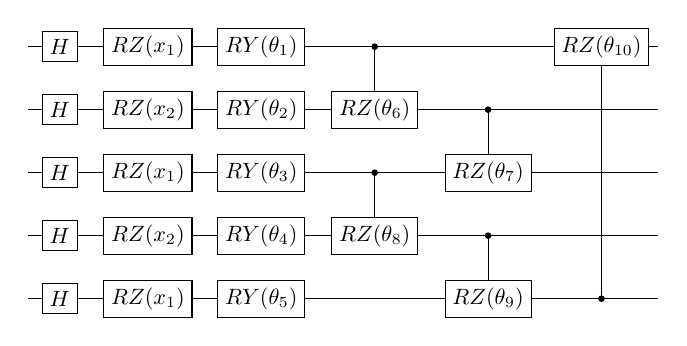
\begin{tikzpicture}[scale=0.8, transform shape]
\begin{scope}
  \node[draw, fill=white] (gate0) at (0.5, 0) {$H$}; %Hadamard
  \node[draw, fill=white] (gate1) at (0.5, -1) {$H$}; %Hadamard
  \node[draw, fill=white] (gate2) at (0.5, -2) {$H$}; %Hadamard
  \node[draw, fill=white] (gate3) at (0.5, -3) {$H$}; %Hadamard
  \node[draw, fill=white] (gate4) at (0.5, -4) {$H$}; %Hadamard
  \node[draw, fill=white] (gate5) at (1.9, 0) {$RZ(x_1)$}; %RZ
  \node[draw, fill=white] (gate6) at (1.9, -1) {$RZ(x_2)$}; %RZ
  \node[draw, fill=white] (gate7) at (1.9, -2) {$RZ(x_1)$}; %RZ
  \node[draw, fill=white] (gate8) at (1.9, -3) {$RZ(x_2)$}; %RZ
  \node[draw, fill=white] (gate9) at (1.9, -4) {$RZ(x_1)$}; %RZ
  \node[draw, fill=white] (gate10) at (3.6999999999999997, 0) {$RY(\theta_{1})$}; %RY
  \node[draw, fill=white] (gate11) at (3.6999999999999997, -1) {$RY(\theta_{2})$}; %RY
  \node[draw, fill=white] (gate12) at (3.6999999999999997, -2) {$RY(\theta_{3})$}; %RY
  \node[draw, fill=white] (gate13) at (3.6999999999999997, -3) {$RY(\theta_{4})$}; %RY
  \node[draw, fill=white] (gate14) at (3.6999999999999997, -4) {$RY(\theta_{5})$}; %RY
  \draw[] (5.5, 0) -- +(0, -1) node[pos=0, circle, fill=black, inner sep=0pt,minimum size=3pt] {{}} node[pos=1, draw, fill=white] (gate15) {$RZ(\theta_{6})$}; %CRZ
  \draw[] (5.5, -2) -- +(0, -1) node[pos=0, circle, fill=black, inner sep=0pt,minimum size=3pt] {{}} node[pos=1, draw, fill=white] (gate16) {$RZ(\theta_{8})$}; %CRZ
  \draw[] (7.3, -1) -- +(0, -1) node[pos=0, circle, fill=black, inner sep=0pt,minimum size=3pt] {{}} node[pos=1, draw, fill=white] (gate17) {$RZ(\theta_{7})$}; %CRZ
  \draw[] (7.3, -3) -- +(0, -1) node[pos=0, circle, fill=black, inner sep=0pt,minimum size=3pt] {{}} node[pos=1, draw, fill=white] (gate18) {$RZ(\theta_{9})$}; %CRZ
  \draw[] (9.1, -4) -- +(0, 4) node[pos=0, circle, fill=black, inner sep=0pt,minimum size=3pt] {{}} node[pos=1, draw, fill=white] (gate19) {$RZ(\theta_{10})$}; %CRZ
\begin{pgfonlayer}{bg}
  \draw (0, 0) -- (10.0, 0);
  \draw (0, -1) -- (10.0, -1);
  \draw (0, -2) -- (10.0, -2);
  \draw (0, -3) -- (10.0, -3);
  \draw (0, -4) -- (10.0, -4);
\end{pgfonlayer}
\end{scope}
\end{tikzpicture}
\end{center}

        \caption{The block from which the \ac{QEK} ansatz is constructed for $N=5$ qubits and $m=2$ features. $\{\theta_j\}_{j=1}^{s=10}$ are the trainable parameters of the kernel and $x_{1,2}$ are the embedded features. The choice of controlled Pauli $Z$ rotations as entangling gates allows us to reduce the circuit depth.}
        \label{fig:circuit_layer}
    \end{figure}
    
    One can interpret the number of qubits $N$ and the number of blocks $L$ as the hyperparameters of the problem, much like the number of neurons per layer and the number of layers in artificial neural networks.
    For each experiment, different hyperparameter values will yield the best fit, depending on the dimension and the complexity of the data.
    For our experiments, we list both the hyperparameters used and results achieved in Tab.~\ref{tab:kernel_experiments}. 
    
    \todo{Should we mention here all the technical details of software and hardware we use?}
    

\subsection{Kernel experiments} \label{ssec:kernel_experiments}
%
    We perform three experiments to evaluate the performance of our trainable kernel without noise. Each experiment follows the following steps:
    \begin{itemize}
        \item Create a data set with balanced labels.
        \item Sample three sets of random kernel parameters.
        \item Fit an \ac{SVM} to the training data using the untrained kernel, once for each set of random kernel parameters.
        \item Report the minimum achieved accuracy and maximum achieved accuracy of the three \acp{SVM}, as tested on the test data. This will be referred to as \emph{untrained accuracy}.
        \item Optimize the kernel parameters via kernel target alignment, initialized at the random parameters with lowest accuracy.
        \item Fit an \ac{SVM} to the train data using the optimized kernel.
        \item Report the achieved accuracy on the test data. This will be referred to as \emph{trained accuracy}.
    \end{itemize}
    Accuracy is defined as the total number of correct classifications divided by the total number of samples. The data sets, used hyperparameters and achieved accuracies are summarized in Tab.~\ref{tab:kernel_experiments} and discussed in more detail below.
%
\begin{table*}
\caption{Kernel experiments and ensemble experiments - data sets, circuit hyperparameters and achieved accuracies} \label{tab:kernel_experiments}
\begin{tabular*}{\textwidth}{c @{\extracolsep{\fill}} ccccccc }
\toprule
 Dataset & samples ($n$) & Width ($N$) & Depth ($L$) & Untrained & Untrained & Trained \\
  & & & & (minimum) & (maximum) & \\ 
  \midrule
 Checkerboard & 60 datapoints & 5 & 8 & 0.52 & 0.52 & 0.97\\  
 Zero vs not-zero & 30 datapoints & 4 & 32 & 0.9 & 0.97 & 0.97 \\
 One vs not-one & 30 datapoints & 4 & 32 & 0.77 & 0.77 & 0.97 \\
 Zero vs one & 10 images (15 datapoints each) & 4 & 32 & NA & NA & 1\\
 Symmetric Donuts & 60 datapoints & 3 & 3 & 0.58 & 0.82 & 0.75  \\
 Symmetric Donuts & 60 datapoints & 4 & 3 & 0.65 & 0.70 & 0.85\\

 \bottomrule
\end{tabular*}
\end{table*}
%
\paragraph{Checkerboard}
    For the checkerboard experiment, performed by simulation on classical hardware, a grid of four by four centroids were laid out. 
    We then used a Gausian distribution to sample datapoints around the centroids, resulting in a total of 30 train- and 30 test-datapoints. 
    The circuit was initialized using five qubits and eight blocks, and random values for the kernel parameter sets. 
    Evaluating this circuit on test data resulted in an accuracy of $0.52$. The optimized kernel achieved an accuracy of $0.97$. The decision boundaries are shown in \ref{fig:datasets_and_decision_boundaries} (c) and (d).
%
\paragraph{Semi-artificial MNIST}
    Moving our experiment closer to real-world data, we now consider MNIST images on using simulation on classical hardware. 
    MNIST contains hand-written digits in images that have dimension 28x28 and a gray-scale from 0 to 255, which we normalize in the range 0 to 1.
    From the MNIST dataset we take $500$ images from both "0" and "1", sample 3 pixel that have a gray-scale value above 0.95, and add all coordinates to sets "zero-base" and "one-base". 
    We now construct the dataset "zero" by taking coordinates in "zero-base", disregarding any coordinates that are also present in "one-base", and follow a similar procedure for our dataset "one". 
    For dataset "non-zero", we take the coordinates that are present both in "zero-base" and "one-base", as well as all remaining coordinates from "one-base".
    We follow a similar procedure for "one". 
    %
    The accuracy of the untrained kernels on "zero vs not-zero" ranged from $0.9$ to $0.97$. 
    Training the kernel on test data starting at the worst-performing parameters raised the accuracy to $0.97$. 
    The untrained kernels on the "one vs not one" set performed worse, with a consistent accuracy of $0.77$. 
    Training the kernel on test data raised the accuracy to $0.97$ again. 
    The decision boundaries are shown in Fig.~\ref{fig:datasets_and_decision_boundaries} (e-h) respectively. 

\paragraph{Symmetric donuts}
    The symmetric donuts dataset consist of 60 train- and 60 test-datapoints, shown in Fig. \ref{fig:datasets_and_decision_boundaries} (i-l).
    Using a shallow circuit, with $3$ blocks on $3$ qubits, we obtain a kernel that has training accuracy of $0.75$, which is higher than the minimum untrained accuracy of $0.58$ but lower than the maximum untrained accuracy of $0.82$. Using $3$ blocks and $4$ qubits, the trained accuracy is $0.85$ which is higher than the maximum untrained accuracy of $0.70$. Furthermore, as can be seen in Fig. \ref{fig:datasets_and_decision_boundaries}, the decision boundaries of the \acp{SVM} are better fitted to the dataset for the trained kernels compared to the untrained kernels for both circuit sizes. As training a kernel using a small circuit already shows an advantage for this dataset, we used this dataset for our hardware experiment \ref{ssec:numerics_hardware}.
    
    
    %
\begin{figure}
\centering
\begin{tabular}{cc}
  \includegraphics[width=0.475\columnwidth]{figures/zero.png} &   \includegraphics[width=0.475\columnwidth]{figures/one.png} \\
 (a) "Zero-base" DS (rotated) & (b) "One-base" DS (rotated) \\[6pt]
 %
 \includegraphics[width=0.475\columnwidth]{figures/checkerboard/checkerboard_random.png} &   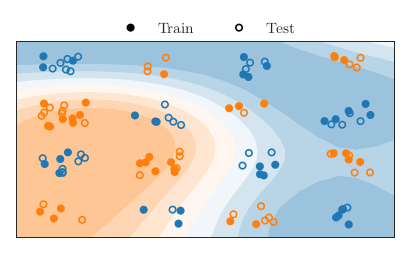
\includegraphics[width=0.475\columnwidth]{figures/checkerboard/trained_checkerboard.png} \\
 (c) "Checkerboard" DBP & (d) "Checkerboard" DBP \\
 - random kernel & - trained kernel \\[6pt]
 %
 \includegraphics[width=0.475\columnwidth]{figures/dataset_MNIST_23_zero_untrained.jpg} &  \includegraphics[width=0.475\columnwidth]{figures/dataset_MNIST_23_zero_trained.jpg} \\
  (e) "Zero vs not-zero" DBP & (f) "Zero vs not-zero" DBP \\
 - random kernel & - trained kernel \\[6pt]
 %
  \includegraphics[width=0.475\columnwidth]{figures/dataset_MNIST_23_one_untrained.jpg} &  \includegraphics[width=0.475\columnwidth]{figures/dataset_MNIST_23_one_trained.jpg} \\
  (g) "One vs not-one" DBP & (h) "One vs not-one" DBP \\
 - random kernel & - trained kernel \\
    \includegraphics[width=0.475\columnwidth]{figures/symmetric_donuts/depth_3_width_3_untrained.png} & 
    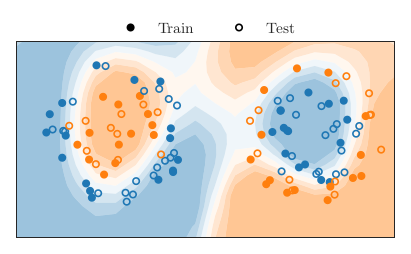
\includegraphics[width=0.475\columnwidth]{figures/symmetric_donuts/depth_3_width_3_trained.png} \\
    (i)  Symmetric donuts DBP & (j) Symmetric donuts DBP \\
    - width 3 depth 3 random kernel & -  width 3 depth 3 trained kernel \\
    \includegraphics[width=0.475\columnwidth]{figures/symmetric_donuts/depth_3_width_4_untrained.png} &  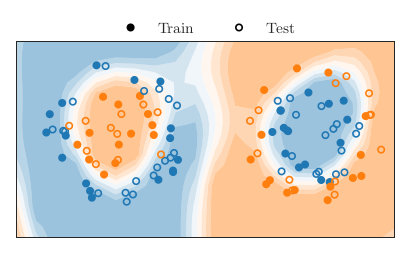
\includegraphics[width=0.475\columnwidth]{figures/symmetric_donuts/depth_3_width_4_trained.png} \\
    (k)  Symmetric donuts DBP & (l) Symmetric donuts DBP \\
    - width 3 depth 4 random kernel & -  width 3 depth 4 trained kernel \\
    
    
\end{tabular}
\caption{Datasets (DS) and decision boundary plots (DBP) for the kernel experiments}
\label{fig:datasets_and_decision_boundaries}
\end{figure}

\subsection{Ensemble experiments} \label{ssec:ensemble_experiments}
    In the previous experiment, we aimed at classifying single pixel coordinates from a combined pool of $500$ images as belonging to a "0" ("1") image or not.
    Here we will show how such classifiers can be combined in an ensemble to classify "zero vs one" by sampling individual MNIST images. %
    To classify an image, we will take the following steps:
    \begin{itemize}
        \item Sample $15$ pixels with gray-scale higher than 0.95 from the image, and store as coordinates.
        \item For each pixel, using the trained kernel classifiers from above,
        \begin{itemize}
            \item Classify "zero" vs "not zero".
            \item Classify "one" vs "not one".
        \end{itemize}
        \item Perform majority vote. Repeat if there is not at least a relative difference of two votes.
    \end{itemize}
    This method allowed us to correctly classify all five "zero" and all five "one" images. 

\subsection{Mitigation and regularization experiments}\label{ssec:numerics_mitigation}

To investigate the effect of the regularization and device noise mitigation techniques introduced in Sec.~\ref{sec:the_effects_of_noise}, we simulate depolarizing noise at the gate execution level, including noise on idling qubits.
We use the checkerboard training data set and circuit previously introduced (also see Tab.~\ref{tab:kernel_experiments}). 
All applied noise channels are single-qubit depolarizing channels on the qubits the corresponding gate acts on.
For a given base noise rate $\lambda_0$, we scale the noise rate for the depolarizing channel linearly with the rotation angle of the specific gate and for idling gates we use $\lambda_0/2$.

For a range of base noise rates $\lambda_0$ and numbers of measurements $M$ per kernel matrix entry, we compute $\tilde{G}_M$.
We then consider any combination of up to three methods with the order \emph{regularize - mitigate - regularize}, including combinations that skip one or two of these steps to post-process $\tilde{G}_M$.
The quality of each mitigation strategy is finally evaluated as the change in alignment with $K$, the noiseless matrix, compared to the raw noisy matrix $\tilde{G}_M$, divided by the deviation of the raw matrix from perfect alignment:
\begin{align}\label{eq:def_quality_postproc}
    q = \frac{\operatorname{A}(\overline{K}_M, K)-\operatorname{A}(\tilde{G}_M, K)}{1-\operatorname{A}(\tilde{G}_M, K)}
\end{align}

Fig.~\ref{fig:relative_improve_postprocessing} shows the improvement $q$ across the base noise rates and numbers of measurements for the best of the $42$ combinations, achieving values between $0\%$ and $43\%$.
For more details on the considered combinations of regularization and mitigation and for the best choice out of those for different noise regimes, refer to App.~\ref{sec:postprocessing_rating}.

Overall, we see that post-processing in general can enhance the quality of the obtained kernel matrix significantly, in addition to other possible mitigation techniques that may reduce the effective sampling and device noise strengths.
At the same time, one has to choose the mitigation and regularization techniques carefully as their quality depends on the noise strengths and does not behave as expected in all regimes. 
If no estimate for the noise levels is available, applying a simple regularization routine like thresholding offers systematic and consistent improvement, but for realistic noise levels, mitigation typically provides even better results (also see Sec.~\ref{ssec:numerics_hardware} and App.~\ref{sec:postprocessing_app}).

When using one of the mitigation techniques one should consider that for $m_{\text{single}}$ only one of the diagonal entries of the kernel matrix needs to be calculated, while multiple (all) diagonal entries are required for $m_{\text{mean}}$ ($m_{\text{split}}$).

\begin{figure}
    \centering
    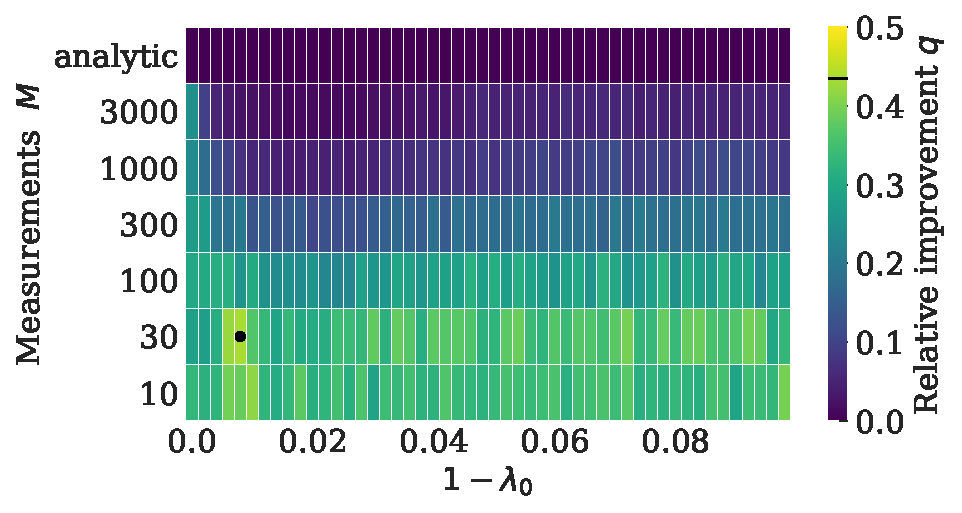
\includegraphics[width=0.48\textwidth]{figures/relative_improvement_postprocessing_Checkerboard_untrained.pdf}
    \caption{Relative improvement $q$ in alignment (see Eq.~\eqref{eq:def_quality_postproc}) for several base noise rates $\lambda_0$ and numbers of measurements $M$ under a realistic noise model.
    We here use the best of our post-processing pipelines $r_\mathrm{SDP}$, which consists of a single step, rated by worst alignment across all noise regimes (for the detailed ranking see App.~\ref{sec:postprocessing_rating}).
    The additional line in the color bar indicates the best relative improvement and the marker in the heatmap shows where it occurs.
    }
    \label{fig:relative_improve_postprocessing}
\end{figure}

    \todo{Explain we run wide instances on simulator and narrow instances on hardware using Pennylane}.

\subsection{Hardware experiments}\label{ssec:numerics_hardware}

We now compute the kernel matrix for the symmetric donuts training data set with the $3$-qubit circuit on a QPU, more concretely on an ion trap device by IonQ.
For the computation we use $M=175$ measurements per kernel matrix entry and measure the diagonal entries for mitigation purposes, summing to about $3.2\cdot 10^{5}$ measurements in total. 
In addition we sample the kernel matrix for smaller $M$ from the measured distribution\footnote{Note that this is not the same as a proper computation on the quantum device with decreased $M$ because we sample from a sample and not from the true distribution directly.}.

Fig.~\ref{fig:ionq_mitigation} shows the alignment $\operatorname{A}(\tilde{G}_M, K)$ of the obtained kernel matrix $\tilde{G}_M$ with the noiseless matrix $K$ as well as the alignment of the post-processed matrix $\overline{K}_M$ with $K$ and the relative improvement $q$ (see Eqn.~\eqref{eq:def_quality_postproc}).
For each measurement number $M$ we show the single best (two best) of the $42$ post-processing pipelines in the lower (upper) plot but note that many of the pipelines yield a quality similar to the best choice.
As expected, the quality of the kernel matrix improves with $M$ and as predicted by our simulation results (see App.~\ref{ssec:numerics_mitigation}), the post-processing methods increase the alignment significantly.
The achieved values for $q$ range between $10.1\%$ and $28.1\%$ with a mean of $15.6\%$.

We note that the pipeline $m_\mathrm{mean},\;r_\mathrm{SDP}$, which is either best or second best in these results on hardware, was correctly predicted by our simulations of depolarizing noise, on a different data set and with different circuit depth and width, see App.~\ref{sec:postprocessing_app}.
This hints at the depolarizing noise model to capture properties of the noise in the QPU that are significant for the kernel matrix computation, and at the post-processing methods to show robust performance across circuit depths, qubit counts and data sets.

In conclusion, our results on the quantum device demonstrate an increased kernel matrix quality based on post-processing, which may allow for improved classification accuracy (also see~\cite{wang2021UnderstandingQEKPower}) or alternatively for reduced measurement budgets while maintaining a fixed classification performance.

\begin{figure}
    \centering
    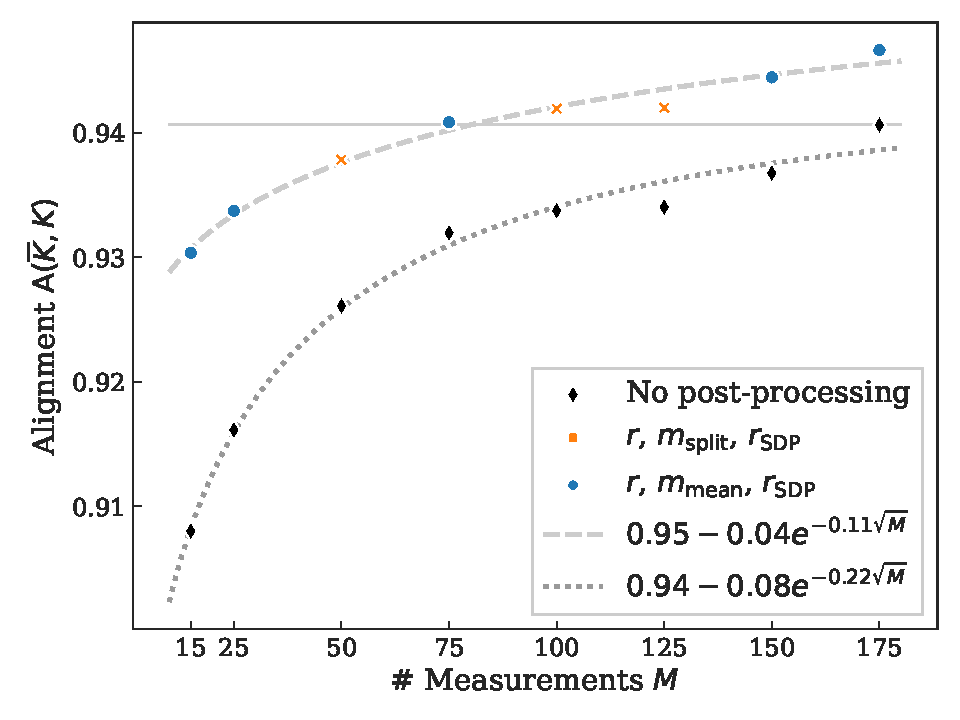
\includegraphics[width=0.48\textwidth]{figures/ionq_mitigation.pdf}
    \caption{Alignment of the kernel matrix measured on the ion trap QPU with the simulated, noiseless kernel matrix for various numbers of measurements $M$ with and without the respective best post-processing pipeline.
    Applying our device noise mitigation $m_\mathrm{mean/split}$, which assumes a simple global depolarizing noise model, and matrix regularization $r_\mathrm{SDP}$ allows for an improved alignment. 
    Alternatively it reduces the required number of measurements, e.g.~to obtain the maximal raw alignment (solid line).
    The bar plot on top displays the relative improvement $q$ (see Eqn.~\eqref{eq:def_quality_postproc}) achieved by the post-processing. 
    }
    \label{fig:ionq_mitigation}
\end{figure}

\section{Summary and Outlook}
\label{sec:summary_and_outlook}

    In this work, we have studied the concept of Quantum Embedding Kernels. After proposing to use quantum embedding circuites as feature maps for kernel-based machine learning, we transferred the concept of kernel target alignment to the quantum setting, with the goal of making good use of well established classical kernel optimization ideas.
    
    Focusing on noise as prominent limitation present in near-term quantum devices, we propose techniques for mitigating depolarizing noise and state concentration results for finite sampling noise.

    Due to the constraint that kernel matrices must be positive semidefinite, dealing with noise is of the utmost importance.
    Therefore, we combine error mitigation techniques with regularization processes that ensure this positive semidefiniteness of the reconstructed kernel matrices.
    Here, we have performed an exhaustive benchmark of all possible combinations of the discussed noise mitigation and regularization techniques and reported what strategy is best at different levels of noise baseline and number of output samples.
    
    As a complement to the theoretical presentation, we have tested these approaches on artificial and semi-artificial datasets.
    We have benchmarked our proposed \ac{QEK} on all reasonable settings: numerical simulations with different levels of noise, a noiseless setting and on actual quantum hardware.

    The goal of this work is to bring attention to the use of trainable Quantum Embedding Kernels, since the field of kernel-based Quantum Machine Learning has seen an important growth recently. It is our hope that this work contributes in expanding its borders towards quantum methods and in convincing more researchers to do so.
    
    This work constitutes a proof of concept with the additional study of the identification and mitigation of certain noise models. We are aware of several possible extensions to these results and invite the reader to take upon them.
    
    To begin with, one could explore the performance of these methods, for instance by comparing different Ansatz families on different datasets.
    Some key objects of study would be the expressivity of different circuits, the optimal choice of hyperparameters (or, alternatively, how one could perform empirical risk minimization successfully), or how one would build gauge invariant kernel functions~\cite{Bronstein2017GeometricDeepLearning}.
    Also, researching the effect of the barren plateau phenomenon \cite{mccleanBarrenPlateausQuantum2018a} is critical, and subsequently the study of (quantum-aware) cost function alternatives to the target alignment.
    
    Furthermore, our results indicate show we can reduce the effects of noise in the sense we can reconstruct a kernel matrix that is closely aligned to the noiseless one.
    This hints at two challenges: firstly, we need strategies on how to proceed if one does not have access to the noiseless matrix and secondly, it remains to be investigated whether the information loss occurring at the reconstruction of the kernel matrix could hinder the optimization process.
    
    Finally, there are additional questions that remain to be answered: can the proposed model be transferred to more general tasks, for instance to unbalanced binary classification, multiple-class classification, or regression? It also remains unanswered whether there exists a way to significantly reduce the computational demands of some steps in the proposed pipeline. The exploration of the benefits of including classical pre-processing of the parameters of data might also lead to additional improvements.

\section*{Acknowledgments}
We wish to thank Xanadu for the hosting of QHACK 2021 where the foundations of this work were laid. We furthermore wish to express our gratitude to both AWS and Sandbox@Alphabet for providing our team with access to quantum hardware and the floq simulator respectively.
We endorse Scientific CO$_2$nduct \cite{conduct} and provide a CO$_2$ emission table in the appendix.

\section*{TODO}
https://arxiv.org/abs/2103.16774


\bibliography{main.bib}

\appendix

\section{Details on post-processing methods}\label{sec:postprocessing_app}
\subsection{Runtimes and output properties}\label{sec:postprocessing_details}
The post-processing methods we introduced in Sec.~\ref{sec:regularization} and~\ref{sec:device_noise_mitigation} differ in their classical and quantum computational cost and in the properties of the output matrix.

The regularization methods $r_\mathrm{Tikhonov}$ and $r_\mathrm{thresh}$ require the computation of the smallest eigenvalue and of the full eigenvalue decomposition respectively, which has classical complexity $\mathcal{O}(n^3)$ with naive methods but more realistically scales like matrix multiplication for relevant sizes with $\mathcal{O}(n^{2.8})$ (Strassen algorithm \cite{strassen1969gaussian})\footnote{If this was to be a bottle neck, the full matrix multiplication may be skipped when multiplying the kernel matrix with vectors only.}.
The worst case scaling for $r_\mathrm{SDP}$ is $\mathcal{O}(n^{3.8})$, again assuming the Strassen algorithm for matrix multiplication and considering that we use $n$ constraints to fix the diagonal entries \cite{lee2015faster, strassen1969gaussian}.
In our experiments on data sets with $60$ data points, the former two methods had negligible computational cost, whereas $r_\mathrm{SDP}$ on average took $0.5s$ for this rather small matrix.
In addition to this large difference in the prefactor, some additional tests for random matrices confirmed a significantly worse scaling of the cost for $r_\mathrm{SDP}$ compared to $r_\mathrm{Tikhonov}$ and $r_\mathrm{thresh}$.

As they only act on the spectrum, $r_\mathrm{Tikhonov}$ and $r_\mathrm{thresh}$ preserve the eigenbasis of the matrix, a potentially relevant property for the classification task.
On the contrary, $r_\mathrm{SDP}$ does not preserve the eigenbasis but ensures that the output kernel matrix has the correct diagonal entries.

For the mitigation methods, additional quantum computation is required in order to determine the diagonal entries, which in turn are used to estimate the depolarizing noise rate(s).
The number of required entries is $1$, $n_\mathrm{mean}\in[1,n]$ and $n$ for $m_\mathrm{single}$, $m_\mathrm{mean}$ and $m_\mathrm{split}$, respectively, which then should be measured $M$ times like the other matrix entries.
While estimating the noise rate(s) has negligible cost, the modification of the matrix requires $\mathcal{O}(n^2)$ classical computation resources\footnote{This may again be improved if we are not interested in the fully computed matrix but e.g.~in multiplying it with vectors, should it become a major part of the resource requirements.}.

Considering Eq.~\eqref{eq:global_lambda_from_G}, we see that $m_\mathrm{single}$ will estimate a negative noise rate for $G_{ii}>1$, and a noise rate above $1$ for $G_{ii}<2^{-N}$, both being unreasonable estimates.
The first condition will only ever be satisfied if a previous post-processing method increased the diagonal element $G_{ii}$ too far, as a QPU will not output measurement probabilities above $1$, and the second condition holds for extremely strong noise only, which suppresses a theoretical value of $1$ to  $2^{-N}$.
For $m_\mathrm{mean}$ ($m_\mathrm{split}$), the same reasoning holds when replacing $G_{ii}$ by the mean of the considered diagonal entries (all the diagonal entries individually), in particular the $\lambda_i(G)$ and $\Lambda_{ij}(G)$ in Eqs.~(\ref{eq:m_split_0}-\ref{eq:m_split_1}) are well-defined noise rates if $2^{-N}\leq G_{ii}\leq 1$ for all $i$.

Even if the estimated noise rate(s) lie in the physically meaningful range $[0,1]$, the mitigation might produce kernel matrix entries that are not valid probabilities and thus can impossibly be the result of a real \ac{QEK} evaluation.
For a particular noisy matrix entry $G_{ij}$, this happens if 
\begin{align}
G_{ij}\not\in \left[2^{-N}\Lambda_{ij}(G)\;, 1-\Lambda_{ij}(G)(1-2^{-N})\right]
\end{align}
where $\Lambda_{ij}(G)$ is defined in Eq.~\eqref{eq:m_split_2} for $m_\mathrm{split}$ and is to be replaced by $\lambda(G)$ for $m_\mathrm{single}$ and $m_\mathrm{mean}$.

In conclusion, even though there are extreme cases in which our methods might transform the noisy matrix into an invalid kernel matrix, we do not expect these problems to play any role because such extreme noise rates likely would render the QPU output useless.

\subsection{Comparison of post-processing pipelines}\label{sec:postprocessing_rating}
There are many combinations of the post-processing techniques to choose from in order to counter device noise and finite sampling errors.

First, we apply a regularization $r_1$, including the option to not modify $\tilde{G}_M$ at all.
Second, we perform device noise mitigation $m$ and third, we regularize again ($r_2$).

For the two regularization steps $r_{1,2}$, we may apply Tikhonov regularization ($r_\mathrm{Tikhonov}$), thresholding ($r_\mathrm{thresh}$) or the \ac{SDP} fixing the diagonal while thresholding ($r_\mathrm{SDP}$), see Sec.~\ref{sec:regularization}.
For the mitigation step, we choose from single noise rate estimation based on a single ($m_\mathrm{single}$) or the mean ($m_\mathrm{mean}$) diagonal entry of $\tilde{G}_M$, and noise rate estimation per feature embedding ($m_\mathrm{split}$), see Sec.~\ref{sec:device_noise_mitigation}.

Naively, this yields $64$ combinations when including the trivial transformation $\operatorname{Id}$, out of which some are identical, e.g.~$\operatorname{Id}, \operatorname{Id}, r_\diamond$ and $r_\diamond, \operatorname{Id}, \operatorname{Id}$.
In addition, there are special pipelines in which methods effectively act like $\operatorname{Id}$:
First, pipelines of the form $r_\mathrm{SDP}, m, r_2$ for which $m$ already receives a positive semi-definite input matrix with correct diagonal entries and thus will estimate the noise rate to be $0$.
Second, some pipelines without mitigation ($r_\textrm{Tikhonov/thresh}, \operatorname{Id}, r_\mathrm{Tikhonov/thresh}$) in which $r_1$ and $r_2$ would be redundant and from which we already excluded the pipelines obeying the first pattern.
Excluding duplicates and these "reducible" pipelines, we obtain $42$ reasonable, distinct pipelines (including $\operatorname{Id}, \operatorname{Id},\operatorname{Id}$) and for each of the outcomes $\overline{K}$ we compute the kernel alignment (see Sec.~\ref{ssec:target_kernel_alignment}) with the noiseless matrix $K$.

In Fig.~\ref{fig:relative_improve_postprocessing} we only showed the best out of the resulting $42$ combinations, rated by the lowest alignment across all base noise rates and numbers of measurements.
This best combination is a single application of $r_\mathrm{thresh}$ (see Eq.~\eqref{eq:thresholding}), not making use of any mitigation or the second regularization step.
However, we note that the influence of sampling noise is rather large in the chosen domains of $M$ and $\lambda_0$, such that the rating by lowest achieved accuracy favors methods that are designed to counter sampling noise, such as $r_\mathrm{thresh}$.

Choosing the pipeline in this way, our post-processing increases the alignment significantly (by up to $43\%$, in the regime of small $M$) and systematically (only negligible deterioration for $M\to\infty$), allowing for an improved estimate of the kernel matrix with fewer measurements.

In Fig.~\ref{fig:best_postprocessing} we evaluate the combinations of regularization and mitigation in more detail and it becomes apparent that the best choice depends on the noise regime.
We immediately see that in the domain of high noise (small numbers of measurements and high noise rate, lower right) the result of our simple ranking is confirmed and thresholding consistently is the best post-processing method (Pipeline $13$).

When increasing $M$ while keeping a high device noise rate, Tikhonov regularization becomes more favorable than thresholding and still no device noise mitigation method is able to improve the matrix further (Pipeline $2$).
This is remarkable because our combinations would allow for multiple processing steps to counter both, sampling and device noise.

For small $\lambda_0$ we observe high variation in which pipeline is best because they yield very similar alignments with the perfect matrix so that statistical fluctuations become relevant.
However, for the majority of these data points with lower noise rates, the combination of single noise rate estimation based on a single or the mean of the matrix diagonal ($m_\mathrm{mean}$) and SDP-based regularization ($r_\mathrm{SDP}$) is best (Pipelines $1$ and $7$).

Finally, for matrices without sampling noise our device noise mitigation techniques combined with Tikhonov regularization are the best choice, delivering far better results than simple regularization (Pipelines $6$ and $10$).
This should not be surprising but indeed confirms that the noise models on which the mitigation techniques are based are able to grasp some of the essential influence the device noise (within our realistic depolarizing noise model) has.
Here the single noise rate estimation seems to be better suited for higher noise rates and $m_\mathrm{split}$ for lower rates.

The complex appearance of Fig.~\ref{fig:best_postprocessing} underlines that the best choice of post-processing depends significantly on the noise level in the device and -- in relation to this level -- how many measurements are used for the kernel evaluation, so one should choose the method carefully.
The benefit of doing so compared to the first, simple rating, is an increase of the best achieved $q$ from $43\%$ to $85\%$ (or even to $90\%$ when considering the results without measurement noise).

\begin{figure*}
    \centering
    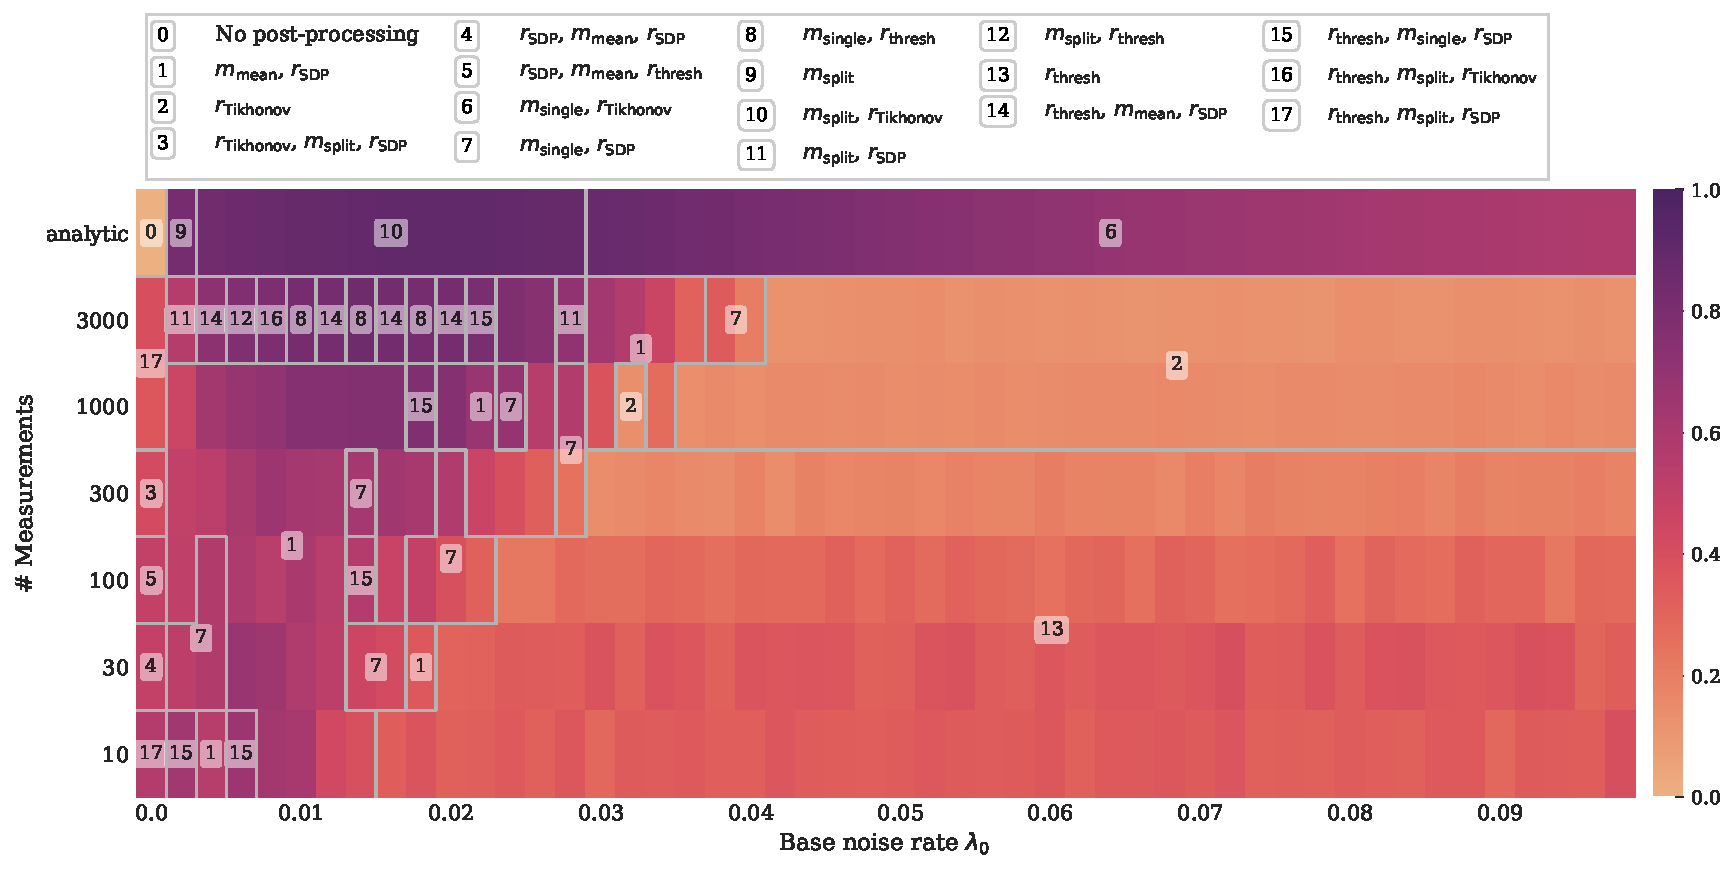
\includegraphics[width=\textwidth]{figures/best_postprocessing_Checkerboard_untrained_relative.pdf}
    \caption{Relative improvement $q$ in alignment between noisy and noiseless kernel matrices as in Fig.~\ref{fig:relative_improve_postprocessing} but for the best choice of post-processing \emph{per point}.
    Solid lines separate areas within which the same combination is best, the circled numbers label the combinations.
    }
    \label{fig:best_postprocessing}
\end{figure*}

Finally, we note that the ranking of the post-processing pipelines based on the alignment of $\overline{K}$ with the noiseless kernel matrix $K$ is not possible in applications that truely require the QPU, as $K$ is not available in this case.
Instead one could evaluate the restored matrices based on their alignment with the ideal target matrix $K^\ast$.
We compared the ranking resulting from this idea with the one presented above and did not find any systematic relations between them, so that this application-oriented surrogate method to reconstruct $K$ may be discarded.
Whether it provides a better kernel matrix for classification is an open question, but if $K^\ast$ was optimal, there would not be any use in computing $K$ from the start.

We conclude that choosing the post-processing in practice remains challenging and requires a systematic analysis of both finite sampling and device noise effects on larger-scale kernel matrices. 

% \begin{align}
%     \calN^2(\rho) &= \calN((1-\lambda) \rho + \lambda \omega)\\
%     &=(1-\lambda) [(1-\lambda) \rho + \lambda \omega]+\lambda\omega\\
%     &=(1-\lambda)^2\rho+[(1-\lambda)\lambda + \lambda]\omega\\
%     &=(1-2\lambda+\lambda^2) \rho + (2\lambda-\lambda^2)
% \end{align}

\section{Additional information on hardware results}

\section{CO\texorpdfstring{$_2$}{2} emission table}
    \begin{center}
    \begin{tabular}[b]{l c}
    \hline
    \textbf{Numerical simulations} & \\
    \hline
    Total Kernel Hours [$\mathrm{h}$]& 42\\
    Thermal Design Power Per Kernel [$\mathrm{W}$]& 5.75\\
    Total Energy Consumption Simulations [$\mathrm{kWh}$] & 42\\
    Average Emission Of CO$_2$ In Germany [$\mathrm{kg/kWh}$]& 42\\
    Total CO$_2$-Emission For Numerical Simulations [$\mathrm{kg}$] & 42\\
    Were The Emissions Offset? & \textbf{Not yet}\\
    \hline
    \textbf{Transport} & \\
    \hline
    Total CO$_2$-Emission For Transport [$\mathrm{kg}$] & 0\\
    \hline
    Total CO$_2$-Emission [$\mathrm{kg}$] & 42\\
    \hline
    \end{tabular}
    \end{center}

% Tiny demo of possible circuit diagrams in fig. \ref{fig:circuit_layer} and here:
% \onecolumngrid
% \input{figures/QEK_ansatz_tikz}


\end{document}

Conventions/Nomenclature/Notation to discuss

- What do we call the data? Training & test set | Training & test data set | Train & Test data
- Kernel matrix or Gram matrix?
- Do we train the kernel, optimize the kernel or optimize the kernel parameters (I guess calling them trainable forces us to train them)? 
- Should we stick to either, trainable or parameterised kernel?
- Do we fit or train an SVM?
- Do we use measurements or shots?
- Is it (finite) sampling noise or error?
- Do we call it Hilbert-Schmidt or Frobenius inner product?
- how to write paramet(e)ri(z/s)ed
\egf{[Parameterised is brit, Parametrized is NA. We said we'd go for NA right?]}
- should we use the acronym package?
- I suggest to not use TA as an acronym but to spell it out or refer to the mathematical term \TA via its symbol.

Math symbols

A               An arbitrary square matrix (n x n) in Hoeffding and alignment section and regularization
A'              An arbitrary PSD matrix
\aa             vectorization of matrix A
\operatorname{A} alignment between to matrices
inequality
B               Second arbitrary matrix in alignment section
b               shift of classification hyperplane
\bb             vectorization of matrix B
$c_i$           Arbitrary coefficient in reals (in Mercer condition)
D               diagonal matrix with spectrum of kernel matrix
$\overline{D}$  postprocessed diagonal matrix 
$\hat{E}$       Noisy Error matrix
$\tilde{E}_M$   Noisy sampled Error matrix
G               noisy kernel matrix (Gram matrix)
$\tilde{G}_M$   noisy, sampled kernel matrix (Gram matrix) with M samples

H               Hadamard gate
\calH           Hilbert space
i,j             typical indices to iterate over range(n)
K               kernel matrix (Gram matrix)
$K_\ttheta$     kernel matrix with explicit parameter dependence
$\overline{K}_M$ noisy, sampled and regularized kernel matrix 
$K^\ast$        (ideal) target matrix
k               kernel (function)
$k_\ttheta$     parametrized (quantum) kernel (function)
$k_RBF$         Gaussian kernel (function) 
L               number of blocks in our QEK template
M               number of samples in statistical estimates (number of matrices)
$M_\mathrm{tot}$ Accumulated number of samples for full matrix (no. of measurements)
m               number of features (dimension of feature space)
$m_{..}$ Mitigation functions
N               number of qubits
n               number of data points and labels in training set
$n_\mathrm{mean}$ number of diagonal kernel matrix entries considered in $m_\mathrm{mean}$
\calN           (generic) noise channel
$\calN_\lambda$ depolarizing noise channel on all qubits

R               Single Pauli rotation gate (in noise section)
$r$             Regularization method
$r_\mathrm{Tikhonov}$ regularization with Tikhonov
$r_\mathrm{thresh}$ thresholding
$r_\mathrm{SDP}$ SDP (thresholding + diagonal fixing)
S               training set
s               typical index to iterate over measurements
\operatorname{TA} target alignment of a kernel
U               State preparation unitary
V               Basis transformation in eigenvalue decomposition
\calV           Noisy Pauli rotation channel
\ww             Normal vector of classification hyperplane
\mathcal{X}     (original) feature space
\xx             feature vector (m-dimensional)
\mathcal{Y}     label space
y               label
\yy             label vector (n-dimensional)

\aalpha         Coefficients in representer theorem to obtain \ww
$\delta$        Probability threshold
$\varepsilon$   Precision parameter/threshold in Hoeffding inequality
$\phi$          feature map 
$\ket{\phi}$    Pure state prepared by embedding circuit 
$\lambda$       Depolarizing rate
$\lambda_0$     Depolarizing base rate
$\rho$          (typically pure state) Density matrix
\ttheta         Trainable parameters of a QEK
$\sigma$        Parameter of RBF/Gaussian kernel
$\omega_\mathrm{min}$ Smallest eigenvalue of a matrix $A$ in Tikhonov regularization.